\documentclass[format=acmsmall, review=false]{acmart}
\usepackage{acm-ec-20}
\usepackage{booktabs} % For formal tables
\usepackage[ruled]{algorithm2e} % For algorithms

\usepackage{subcaption}
\newcommand{\xhdr}[1]{\vspace{1mm} \noindent{\bf #1}}

\renewcommand{\algorithmcfname}{ALGORITHM}
\SetAlFnt{\small}
\SetAlCapFnt{\small}
\SetAlCapNameFnt{\small}
\SetAlCapHSkip{0pt}
\IncMargin{-\parindent}

% Choose a citation style by commenting/uncommenting the appropriate line:
%\setcitestyle{authoryear}
\setcitestyle{acmnumeric}

\newtheorem{finding}{Finding}

% Title. Note the optional short title for running heads. In the interest of anonymization, please do not include any acknowledgements.
\newcommand\PaperTitle{Deconstructing the Filter Bubble: \\ Consumer Decision-Making and Recommender Systems}
\title[\PaperTitle]{\PaperTitle}

% Anonymized submission.
\author{Submission 20}

% Abstract. Note that this must come before \maketitle.
\begin{abstract}
We study a model of user decision-making in the context of recommender systems via numerical simulation. We explore the extent to which two issues traditionally associated with recommender systems -- \textit{filter bubbles} and \textit{user homogenization} -- can be attributed to recommendation systems. In our model users face a sequential decision problem under uncertainty and there are informational spillovers where a user consuming a product and learning how she values it reduces uncertainty and provides information about similar products. We find that this generates behavior consistent with filter bubble effects -- where users consume increasingly similar items over time -- and that recommendation can help alleviate these effects, as has been found in the empirical work of Nguyen et al. (2014). However, we find that recommendation, while alleviating filter bubble effects, leads to an increase in user homogeneity. Our results highlight the path-dependence of user choice in environments where recommender systems are deployed.
\end{abstract}

\begin{document}

\maketitle


% Paper body
\section{Introduction}

Users in many online platforms face difficult decision problems as they have to sort through the vast choice sets present in these markets. For instance, users have to select from thousands of movies on Netflix, millions of products on Amazon, and billions of videos on YouTube. A common remedy introduced by online platforms has been to deploy \textit{recommender systems}, which have become critical for assisting users in making consumption decisions. These systems provide users with information and recommendations to allow them to make more informed consumption decisions. These systems have been shown to be influential in steering consumer choice with 75\% of movies watched on Netflix and 35\% of page-views on Amazon coming from recommendations.\footnote{MacKenzie et al. (2013, Oct.),  How retailers can keep up with consumers. 
\url{https://www.mckinsey.com/industries/retail/our-insights/how-retailers-can-keep-up-with-consumers}. 
Retrieved on October 3, 2019.}
\par 
Despite evidence of the power of these systems in determining user choice, we have little theoretical understanding of how users make choices in these markets and how recommender systems shape these choices. Understanding this has become increasingly important as a number of concerns have emerged regarding the broader social and economic consequences of such systems. There have been claims that YouTube's recommendation algorithm unintentionally led to the radicalization of many individuals,\footnote{Friedersdorf (2018, Mar. 12), YouTube Extremism and the Long Tail, 
\textit{The Atlantic}. 
\url{https://www.theatlantic.com/politics/archive/2018/03/youtube-extremism-and-the-long-tail/555350}. Retrieved on October 3, 2019.} 
that personalized recommender systems lead users into \textit{filter bubbles} 
where they effectively get isolated from a diversity of viewpoints or content 
\cite{pariser2011filter}, and that personalized recommender systems may also lead users to become increasingly homogenized at the same time \cite{chaney2018algorithmic, hosanagar2013will}. Furthermore, an emerging worry is that recommender systems can be utilized to steer consumer choice towards products more profitable for online platforms to the detriment of consumer welfare and the overall competitiveness of such markets \citep{aridor2020recommender, bourreau2018streaming, DeCorniereTaylor2019RAND}. Finally, there has emerged a burgeoning literature that focuses on understanding how recommender systems themselves can acquire information about product quality from the choices of self-interested consumers \cite{kremer2014implementing, che2017recommender,frazier2014incentivizing,mansour2015bayesian}. 
\par
While these issues are important and wide-reaching, it is hard to make progress on them without a model of user choice with foundations in economic decision theory and psychology. In this paper we provide such a model of user preferences and choice in these markets and study how the introduction of recommendation affects user choice. Our primary focus is on utilizing our model to understand the extent to which recommender systems lead individual users into filter bubbles and homogenize across user consumption choices. We rationalize existing empirical work on these topics and provide an argument for the underlying mechanisms behind such effects. We also discuss how our model can shed light on how recommender systems can be utilized to steer choice and affect the long-term consumption patterns of users. Finally, our model provides a direction for making progress on an open question in the literature on incentivizing exploration in recommender systems on how to incorporate realistic models of user choice into such models (e.g. \citep{immorlica2018incentivizing}).

\xhdr{Our Model} We consider a model of user choice that has the following components.
\par
The first component of our model is that users sequentially consume items and face large choice sets. In our setting of interest users are long-lived, but they only consume a small fraction of this choice set over their lifetime.
\par
The second component of our model is that users have \textit{uncertainty} about their valuation of the different items. This is motivated both by the fact that many markets where recommender systems are deployed contain experience goods, whose true value can only be learned after consumption, and the fact that such uncertainty is why recommender systems exist in the first place. Thus, users face a sequential decision-making problem under uncertainty.
\par 
The third, and key, component of our model is that consumption of an item reveals information that changes user beliefs about the valuation of similar items. Unlike in standard sequential decision-making problems, in our model once an item is consumed all uncertainty about its valuation is resolved. This valuation provides information for consumers that enables them to update their beliefs about similar items. This exploits the fact that the valuations of similar items are correlated which assists users in navigating the vast product space. The idea that users make similarity-based assessments to guide their choice has grounding in theoretical work in decision theory \cite{gilboa1995case} and empirical evidence of how users navigate large choice sets \cite{schulz2019structured}.
\par 
The fourth component of our model is that recommendation provides users with information about the true valuations. We model the realized valuations as being a weighted sum of a common-value and an idiosyncratic component. This formulation gives a stylized notion of predictability of user preferences where the idiosyncratic component is inherently unpredictable given other individuals' preferences and the common-value component is what the recommender can learn from previous users' data. We suppose that the recommender knows the common-value component for each item and combines it with individuals' beliefs over the product space when designing personalized recommendation.

\xhdr{Main Findings}
Our first set of results focuses on understanding to what extent recommender systems lead users into filter bubbles and how such filter bubbles may naturally arise. The standard notion of filter bubbles is that, over time, user consumption becomes increasingly concentrated on narrower and narrower parts of the product space, leading to a decreasing distance between subsequent consumed items over time. However, empirical work such as \cite{nguyen2014exploring}, finds that user consumption choices over time naturally exhibit such filter bubble effects even without recommendation and that, in fact, recommender systems mitigate such effects. The results of our model are in line with these empirical results and give a clear intuition as to why such effects arise and why recommendation mitigates them to some degree.
\par
We first find that when there is no correlation between the valuations of goods there is no reason for filter bubble effects to arise, regardless of the information that users have on the valuations of the products. However, once there is a correlation between the true valuations of the items then such filter bubble effects arise even without recommendation.\footnote{The fact that in many environments where recommender systems are deployed the true valuations of items are correlated makes this the most relevant case to consider. Indeed, the core idea behind standard content-based recommendation methods relies on this fact as these methods determine recommendations based on finding similar items to those that a user has consumed before and enjoyed \citep{adomavicius2005toward}.} The intuition is that, users initially have uncertainty about their true valuations and initial consumption of items leads them to update their beliefs strongly about the average utility of nearby items. When a user finds an item that has high realized utility, this induces her to update her beliefs positively about the realized utility of nearby items which leads to  the consumption of these items. Thus, without recommendation users increasingly consume items in this portion of the vast product space since they never get information about items in different parts of the product space. This learning spillover not only induces positive updates about the average utility of the item, but also reduces the level of uncertainty they have about these items. Thus, this effect is further amplified when users are \textit{risk-averse}. This is a standard concept from decision theory by which, all else being equal, users have a preference for items with lower uncertainty to those with higher uncertainty.
\par 
We then investigate whether the introduction of recommendation either mitigates or amplifies this effect. Recommendations could potentially make matters worse: providing information about the common value of the items when this value is correlated could intensify the extent of local consumption. However, in line with existing empirical work, we find the opposite - that recommendation partially mitigates this narrowing effect - since the revelation of the common value component allows for users to escape being stuck in portions of the product space due to lack of information about other portions of the product space.
\par
\xhdr{Additional Findings} We further explore the diversity of the overall set of items that users consume. Encouraging consumption diversity is increasingly a common goal of many recommender systems \cite{castells2015novelty, kunaver2017diversity}, which is reasonable since it could be expected that higher diversity is associated with more intense search and therefore higher welfare. However, we find that, without recommendation, higher diversity of items consumed does not ensure higher welfare. This is due to the fact that high consumption set diversity in our model can arise from a sequence of bad realizations, which leads to very intense search over very different parts of the product space and high consumption diversity but very low welfare. However, discovering a sweet spot leads to highly rewarding local search and very low diversity. Thus, contrary to what a natural intuition could suggest, we find that consumption set diversity is not by itself a useful measure for understanding the impact of recommender systems on user welfare.
\par
We then turn to the extent to which recommendation leads to increasing user homogenization. In our context we define homogenization as the degree of similarity between the set of consumed items across individuals. We find that, without recommendation, there is very little homogenization as users are effectively all doing their own random exploration around the product space. In the ex-post utility maximizing consumption path (i.e. the consumption path the user would have taken if all uncertainty had been resolved) we find that some degree of homogenization is optimal. However, we find that while recommendation leads to an increase in consumer welfare, it concentrates user consumption choices in the same portions of the product space where there is a high common-value component. As a result, it leads to a substantially higher homogenization when compared both to the no recommendation and ex-post utility maximizing consumption path.
\par 
One implication from our model is that the user consumption paths have a clear path-dependence since the consumption of an item today influences the information a user has tomorrow which further influences consumption choices tomorrow. This is important for the debate regarding the extent to which recommender systems can be utilized to steer consumer choice as most of the literature analyzes this in a static context. However, this path-dependence implies that such platform steering can have dynamic consequences as steering towards certain items today can shape the long-run consumption choices of users. 

\xhdr{Related Work.} 
The first set of related works studies the extent and implications of filter bubbles. \cite{pariser2011filter} first informally described the idea of the ``filter bubble'' which is that online personalization services would lead users down paths of increasingly narrower content so that they would effectively be isolated from a diversity of viewpoints or content. Following this a number of empirical studies, done in various disciplines, have since studied the extent to which this phenomena exists in a wide range of contexts \cite{flaxman2016filter,hosanagar2013will,moller2018blame,nguyen2014exploring}. The most relevant to our study is \cite{nguyen2014exploring} who study whether this effect exists with recommender systems in the context of movie consumption. They find that even users whose consumption choices are not guided by recommendations fall into behavior consistent with ``filter bubbles'' and that recommender systems can actually increase the diversity of the content that users consume. To our knowledge there are no theoretical models that rationalize these empirical findings and our paper provides a theoretical framework through which to view this problem. Further, our paper provides a clear mechanism at play that drives such effects and how recommendation interacts with them.
\par 
Another set of papers have examined whether recommender systems can lead users to become increasingly homogenized or consume similar content as each other. \cite{celma2008hits, treviranus2009value} show that incorporating content popularity into recommender systems can lead to increased user homogenization. \cite{chaney2018algorithmic} show how user homogenization may arise from training recommender systems on data from users exposed to algorithmic recommendations. \cite{fleder2009blockbuster} argues that homogenization can increase due to a recommendation bias towards popularity that arises from lack of information about items with limited consumption histories. Our model leads to similar results as previous theoretical and empirical work where recommender systems lead to increased user homogenization. However, the mechanisms behind this from our model differ from existing work as homogenization arises due to the fact that recommendation leads users to coordinate their consumption decisions in certain portions of the product space.
\par 
Our model of decision-making draws from work in decision theory and psychology. \cite{schulz2019structured} empirically studies how individuals solve sequential decision-making problems under uncertainty in large choice sets in the context of mobile food delivery orders. They find that individuals engage in similarity-based generalizations where learning about the realized value of a particular good provides them with information about similar items. We incorporate this finding into our model in a stylized manner where a single parameter controls the degree of information spillovers. \cite{gilboa1995case} considers a model of case-based decision making where choices are made based on information from previously experienced choice problems that are similar to the one faced by the decision-maker. However, while conceptually related, our model incorporates this idea in a different manner by utilizing Bayesian reasoning as opposed to a weighted sum of previous similar choice problems. \cite{hodgson2019horse} consider a similar model as ours where users engage in ``spatial learning'' and exploit the correlation of their preferences in the environment, but consider it in the context of search for a single item as opposed to consumption of multiple items. \cite{bronnenberg2016zooming} empirically show that users engage in a ``zooming in” search strategy in terms of the information they acquire about products before purchasing and only end up acquiring information about a small set of products in a large product space. Finally, \cite{chen2013human} surveys work that has studied decision-making models in the context of recommender systems, though to our knowledge none of these papers study user decision making over time or study filter bubble and homogenization issues.


\section{Our Model and Preliminaries}
\subsection{Preliminaries on Expected Utility Theory}
\noindent For every item $n$ in the product space $\mathcal J$, we assume that each user $i$ assigns a monetary equivalent $x_{i,n} \in \mathbb R$ to the experience of consuming it. Each user can value the same item differently. However, we assume that users have the same utility over money, given by a utility function $u: \mathbb R \to \mathbb R$, strictly increasing and continuous. So, ex-post, the value of item $n$ for user $i$ is given by $u(x_{i,n})$ However, before consuming the item, the user does not know exactly how she will value it. In particular, even users that will end up having the same ex-post valuation of item $n$ may differ in their ex-ante valuation because they hold different beliefs about it. We denote by $p_{i}$ the beliefs item $i$ has about how she will value each of the items in the product space. Note that this implies that consuming item $n$ is the same as taking a gamble. Each user evaluates the item according to the associated expected utility associated with the item, i.e. $U_i(n)=\mathbb E_{p_i}[u(x_n)]$. 
\par

Risk aversion captures the how different users react to the risk associated to a particular consumption opportunity. It is formalized as follows: a given gamble $x$ takes real values and follows distribution $p$. Then, for every gamble $x$, there is a certain amount of money that makes the user indifferent between taking the gamble or taking the sure amount of money. This sure amount of money is called the \textit{certainty equivalent} of gamble $x$ and is denoted as $\delta(x)$. A user $i$ is more risk-averse than another user $j$ when for every gamble $x$, user $i$ requires a lower value to give up the gamble when compared to user $j$, i.e. $\delta_i(x)$. Therefore, a more risk-averse user is more willing to avoid the risk of taking the gamble. We assume that the utility function takes a flexible functional form $u(x)=1-\exp(-\gamma x)$ for $\gamma\ne0$ and $u(x)=x$ for $\gamma=0$ -- known as constant absolute risk-aversion preferences (from hereon CARA). Higher $\gamma$ implies higher risk-aversion with $\gamma=0$ corresponding to the risk-neutral case and $\gamma>0$ to the risk-averse one. Our formulations here follow standard economic decision-theory (see \cite{mas1995microeconomic} for a textbook treatment of these topics).
\par

\subsection{Model}
\par
\xhdr{Users.} We consider a set of users $I$ where each user $i \in I$ faces the same finite set of $N$ items $\mathcal J = \left\{0,1,...,N-1\right\}$. For simplicity, we assume that users only derive pleasure from item $n \in \mathcal{J}$ the first time they consume it.
\par

We denote by $x_{i,n}$ user $i$'s realized value from consuming item $n$. In particular, we consider that the realized value derived from a given item can be decomposed in the following manner: $x_{i,n}= v_{i,n} + \beta v_n$, where $v_{i,n}$ denotes an idiosyncratic component -- i.e. user $i$'s idiosyncratic taste for product $n$ --  and $v_{n}$, a common-value component. One can interpret $v_n$ as a measure of how much item $n$ is valued in society in general and, in a sense, $v_{i,n}$ denotes how $i$ diverges from this overall ranking. The scalar $\beta \in \mathbb{R}_{t}$ denotes the degree to which valuations are idiosyncratic to each user or common across users. If $\beta=0$, it is impossible to generate meaningful predictions of any one's individual preferences based on others, while if $\beta$ is large, every individual has similar preferences.
\par
Stacking values in vector-form, we get the vector of values associated with each item 
$${\left(x_{i,n}\right)}_{n \in \mathcal{J}}=:X_i =V_i+ \beta V $$
where $V_i ={\left(v_{i,n}\right)}_{n \in \mathcal{J}}$ and $V={\left(v_{n}\right)}_{n \in \mathcal{J}}$.
\par
\xhdr{User Decision-Making.}
We assume the user makes $T$ choices and therefore can only consume up to $T$ items, where $T$ is a small fraction of $N$. This captures the idea that users are faced with an immense choice set but that ultimately they end up experiencing (and learning) about just a small fraction of it. Since this is a sequential decision-making problem under uncertainty, in principle users face an exploration-exploitation trade-off. However, for tractability, we impose that users are myopic and every period consume the product that they have not yet tried ($n_i^t$) that gives them the highest expected utility given the information from past consumption offers ($C_i^{t-1}=(n_i^1,...,n_i^{t-1})$) and their initial beliefs.
\par
\xhdr{User Beliefs.} We assume that all the true realized values are drawn at $t = 0$. However, users do not know the realized values before consuming an item, but rather have beliefs over the realized utilities.
Formally, user $i$ starts with some beliefs about $X_i$, namely that the idiosyncratic and common-value parts of the valuations are independent -- $V_i \perp \!\!\! \perp V$ -- and that each is multivariate normal 
\begin{enumerate}
\item $V_i \sim \mathcal N (\overline V_i, \Sigma_i)$ 
\item $V \sim \mathcal N(\overline V, \Sigma)$ with $\overline V =0$
\end{enumerate}
We impose the normality assumption for two reasons. The first is that this allows for simple and tractable belief updating. The second is that it allows us to incorporate an easily interpretable correlation structure between the items. The precise formulation of $\Sigma$ and $\Sigma_i$ that we consider is defined below when we discuss user learning.
\par
Keeping with the assumption that $V_i$ represents idiosyncratic deviations from $V$, we assume that, on the population level, prior beliefs $\overline V_i=\left(\overline v_{i,n}\right)_{n \in \mathcal{J}}$ are drawn independently from a jointly normal distribution, where $\overline v_{i,n} \sim \mathcal N (0, \overline \sigma^2)$ are independent and identically distributed. These $\overline v_{i,n}$ denote the prior belief that individual $i$ holds about her valuation over item $n$. As people are exposed to different backgrounds, their beliefs about how much they value a given item also varies and $\overline v_{i,n}$ denotes this idiosyncrasy at the level of prior beliefs.
\par

We assume users are expected utility maximizers. User $i$'s certainty equivalent for item $n$, the sure value that makes user $i$ indifferent between it and consuming the item $n$, conditional on the consumption history, is given by
$\delta_{i}(n)\mid C_i^{t-1}=\mu_n-\frac{1}{2}\gamma \Sigma_{nn}$, where $\mu_n$ and $\Sigma_{nn}$ are the expected value and variance for item $n$ that the user has given their initial beliefs and consumption history up until time $t$. Note that this expression is known to be the certainty equivalent for CARA preferences in a Gaussian environment \cite{mas1995microeconomic}.

\xhdr{User Learning}
When a user consumes an item $n$ she learns the realized value for that item. In our model, we incorporate the idea that learning the value of item $n$ gives a user information about similar items. 
%This is drawn from recent empirical evidence in \cite{schulz2019structured} that consumers learn how to navigate large choice sets using similarity-based generalization. 
We assume that learning about the value of item $n$ reveals more about the value associated to items that are closer to it, which captures the idea that trying an item provides more information about similar items than about dissimilar ones.
\par
In order to have a well-defined notion of similarity we need to define a distance function between items, which we define as $d(n,m):=\min\{ \lvert m - n \rvert ,N - \lvert m - n \rvert \}$ where $m$ and $n$ are indices of items in $\mathcal{J}$. This distance function is not intended to model the intricacies of a realistic product space, but instead to provide a stylized product space to help us understand the effects of informational spillovers on user behavior. We consider that the entry of $n$-th row and the ($m$)-th column of $\Sigma_i$ is given by $\sigma_i^2 \rho^{d(n,m)}$, and that of $\Sigma$ is given by $\sigma^2 \rho^{d(n,m)}$. The scalar $\rho \in [0,1]$ therefore impacts the covariance structure: a higher $\rho$ implies that learning the utility of $n$ is more informative about products nearby. Informativeness, for any $\rho \in (0,1)$, is decreasing in distance. The particular distance function that we utilize leads to this covariance structure being simple, where the $(n,n+1)$-th entry in the covariance matrix is $\sigma^{2} \rho$, the $(n,n+2)$-th entry is $\sigma^{2} \rho^2$, etc. \footnote{This exponential decay correlation structure can be related to the tenet of case-based similiartiy of Gilboa and Schmeidler (2008, MSS) for an axiomatization of exponential similarity.}
\par
The precise updating rule is as follows. Recall that at time $t$ the user's consumption history is given by $C_{i}^{t}$ and we denote the utility realizations of these items as $c_t$. We denote $\mu_t$ as the initial mean beliefs the user has over the items in $C_{i}^{t}$ and $\mu_{N-t}$ as the initial mean beliefs the user has over the remaining $N-t$ items, $\mathcal{J} \setminus C_{i}^{t}$. We partition the covariance matrix as follows:
\[ \Sigma =  \left( \begin{array}{cc}
\Sigma_{(N-t, N-t)} & \Sigma_{(N-t,t)} \\
\Sigma_{(t,N-t)} & \Sigma_{(t,t)}
\end{array} \right)
\]
Thus, after consuming the items in $C_{i}^{t}$ the resulting beliefs over the remaining items are given by $\mathcal{N}(\bar{\mu}, \bar{\Sigma})$ where $\bar{\mu}$ and $\bar{\Sigma}$ are as follows:
\begin{align*}
\bar{\mu} \mid c_t = \mu_{N-t} + \Sigma_{(N-t,t)} \Sigma_{(t,t)}^{-1}(c_t - \mu_t) \\
\bar{\Sigma} \mid c_t = \Sigma_{(N-t,N-t)} - \Sigma_{(N-t,t)} \Sigma_{(t,t)}^{-1} \Sigma_{(t,N-t)}
\end{align*}
\begin{figure}[t]
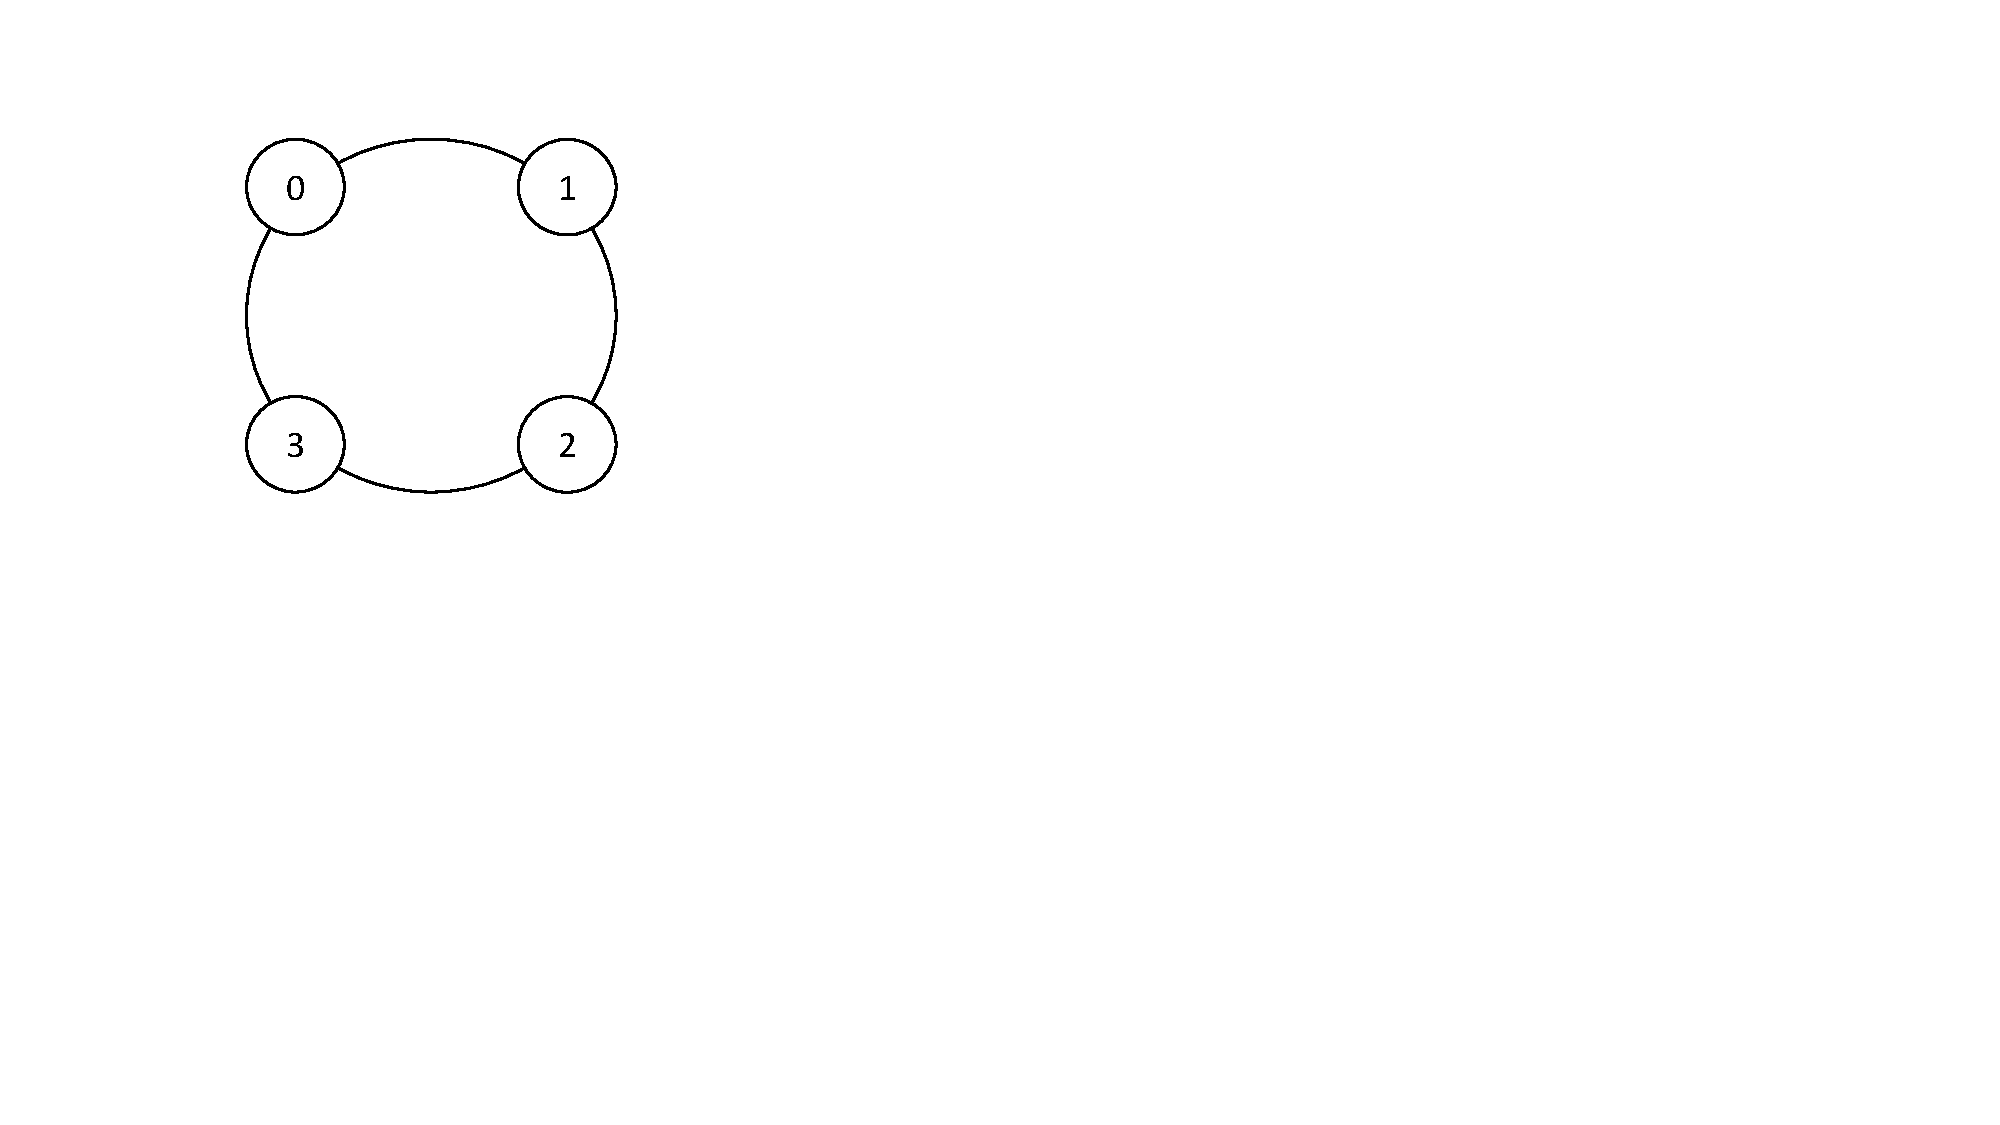
\includegraphics[width=.3\linewidth]{figures/Example-Bubbles.pdf}
\captionof{figure}{Illustrative Example}
\label{fig:illustrative_example}
\end{figure}

\xhdr{An Illustrative Example} We illustrate the main intuitions of our model with a simple example. Suppose that there are four items: 0, 1, 2, 3. The items are in different places of the product space, where 0 is close to 1 and 3 but more distant from 2, as shown in Figure \ref{fig:illustrative_example}. The initial beliefs are given as follows:
\[ \mu = \left (\begin{array}{c}
\mathbb{E}[x_0] \\
\mathbb{E}[x_1] \\
\mathbb{E}[x_2] \\
\mathbb{E}[x_3]
\end{array}  \right) = \left (\begin{array}{c}
0 \\
0\\
0 \\
0
\end{array}  \right), \Sigma =  \sigma^{2} \left( \begin{array}{cccc}
\rho^{0} & \rho^{1} & \rho^{2} & \rho^{0} \\
\rho^{1} & \rho^{0} & \rho^{1} & \rho^{2} \\
\rho^{2} & \rho^{1} & \rho^{0} & \rho^{1} \\
\rho^{1} & \rho^{2} & \rho^{1} & \rho^{0} \\
\end{array} \right)
\]
In period 1, every item is ex-ante identical since they have the same mean and variance and so suppose that the user breaks the tie arbitrarily and consumes item 0. The underlying correlation structure implies that upon observing that $x_0=y$ the user will update beliefs about the remaining 3 items according to the previously specified updating rule. For concreteness, we suppose that $\sigma = 1$ and $\rho = 0.5$, but the intuitions hold for any value of $\sigma$ and $\rho > 0$. First, we consider the case when $y = 0.5 > 0$. The resulting beliefs after observing $y$ are then as follows:
\[ \bar{\mu} =   \left (\begin{array}{c}
\mathbb{E}[x_1] \vspace{0.15cm} \\
\mathbb{E}[x_2] \vspace{0.15cm} \\
\mathbb{E}[x_3]
\end{array}  \right) =\left (\begin{array}{c}
\rho y  \vspace{0.15cm} \\
\rho^{2} y  \vspace{0.15cm} \\
 \rho y \\
\end{array} \right) =
\left (\begin{array}{c}
\frac{1}{4} \vspace{0.15cm} \\
\frac{1}{8}  \vspace{0.15cm} \\
\frac{1}{4}
\end{array}  \right), \bar{\Sigma} =  \left( \begin{array}{ccc}
\frac{3}{4} & \frac{3}{8} & 0 \vspace{0.15cm} \\
\frac{3}{8} & \frac{15}{16} & \frac{3}{8} \vspace{0.15cm}  \\
0 &\frac{3}{8} & \frac{3}{4}  \\
\end{array} \right)
\]
Thus, upon learning $y$, the user updates beliefs about the remaining items. Note that $\mathbb{E}[x_1] = \mathbb{E}[x_3] > \mathbb{E}[x_2]$ since item 0's value is more informative about similar items' values, items 1 and 3, than items further way in the product space such as item 2. Moreover, $\bar{\Sigma}_{11} = \bar{\Sigma}_{33} < \bar{\Sigma}_{22}$ as the uncertainty about items 1 and 3 is further reduced compared to item 2. Thus, since $y > 0$, the user in the next period will consume items nearby to item 0 since, even though initially she believed that all items had the same mean, the spillover from consuming item 0 leads her to believe that items 1 and 3 have higher expected valuations. Since both the mean is higher for these items and the variance is lower, the user will consume items 1 and 3 regardless of her risk aversion levels.
\par 
Suppose instead that item 0 ends up having a negative valuation so that $y = -0.5 < 0$. This results in $\mathbb{E}[x_1] = \mathbb{E}[x_3] = -\frac{1}{4} <  -\frac{1}{8} = \mathbb{E}[x_2]$ with $\bar{\Sigma}$ remaining the same as when $y = 0.5$. In this case the risk-aversion levels of the user determine the choice in the next period. If the user is risk-neutral ($\gamma = 0$), then she will go across the product space to consume item $2$ in the next period since it has a higher expected value. However, if she is sufficiently risk-averse then she still may consume item $1$ or $3$ since her uncertainty about these items is lower than item $2$. In particular, this will happen when 
\begin{align*}
\delta(3) = \delta(1) = \rho y - \frac{1}{2} \gamma \bar{\Sigma}_{11} > \rho^{2} y - \frac{1}{2} \gamma \bar{\Sigma}_{22} = \delta(2)
\end{align*}
Given the aforementioned parametrization and $y = -0.5$, the user will consume item $1$ or $3$ when $\gamma > \frac{4}{3}$ and will consume item $2$ when $\gamma < \frac{4}{3}$. Thus if the user is risk averse enough, then she might be willing to trade-off ex-ante lower expected values for lower risk and stick to consuming nearby items just because these items have lower uncertainty. 
\par 
This example illustrates the main mechanisms in our model that can lead to excessive consumption of similar items. Once the user finds items in the product space with high valuations she will update her beliefs positively about items in this portion of the product space and continue consuming these items regardless of her level of risk aversion. However, this same updating leads to a reduction in uncertainty of these items and so, if she is sufficiently risk-averse, she still may continue consuming items in this portion of the product space, even if she has bad experiences with them, since they are perceived to be less risky. 
\par

\xhdr{Recommendation.}
Our model of recommendation is stylized in order to provide qualitative insights into how recommendation shapes behavior, instead of focusing on the details of how recommender systems are implemented in practice. We model recommendation as giving users information about the valuation of the products.
\par

We will consider three cases. The case of primary interest is \textit{recommendation} where the recommender observes values accrued and knows $V$ but does not know neither $V_i$.\footnote{We do not consider the acquisition of information for the recommender to know $V$ and suppose that she has sufficient data to learn $V$ with arbitrary precision at $t = 0$.} However, the recommender does know the users' beliefs $\bar V_i$. Thus, at any given period, the recommender provides a personalized recommendation that combines the knowledge of the common value component $V$ with the user beliefs $\bar V_i$. Knowing the user's beliefs about her valuation of each item become crucial in this case: just providing the user with information about $V$ may change the user's original ranking, but, without considering the user's beliefs, she will not necessarily follow the recommendation.\footnote{The notion of recommendation that we consider is idealized where the recommendation does the Bayesian updating for users. As users face a very difficult and costly Bayesian updating instance, a useful recommendation system provides recommendations taking into account this aspect and combines the history of past consumption and value realizations with the user's beliefs. 
An alternative that is equivalent would be the recommender simply providing $V$ without knowing $V_i$. In this case, the recommendation will be that the user $i$ chooses $r_{i,t} \in \arg \max_{n\in \mathcal J\backslash C^T_i} \mathbb E[u(x_n) \mid C_i^T]$
but we assume the recommender provides full information about $V$. For instance, the recommender could display the whole distribution of utilities reported by other users or even its average, which is a good proxy for the common value component. It is possible for the recommender to only recommend the best item given such information, that is, the item with highest common value component. However, in that case, recommending only a single item generates costly Bayesian updating to the user and provides little guidance as to what she should indeed pick as the common value might be of little importance when compared to the idiosyncratic component. Therefore, we assume that the recommender reports the whole $V$, which results in higher expected welfare in choices and is not costly to implement.
The results would be equivalent, but this would shift the burden of Bayesian updating to users.}
\par

We further consider two cases that serve primarily as benchmarks. The first is \textit{no recommendation}, where users get no additional information about values and make consumption choices based on their beliefs and consumption history. This gives us a benchmark as to how users in our model would behave \textit{without} recommendation so that we can analyze what changes with the introduction of recommendation. The second is the \textit{oracle recommendation} where the recommender knows the true realized utility of each good for each user and can therefore recommend the best remaining good in every period. This gives us a full information benchmark, which is the optimal consumption path for a user if all uncertainty about their preferences was resolved. Comparison to the oracle regime benchmark provides an analog to the standard regret measures utilized in the multi-armed bandit literature, which look at the difference in the expected value of the ex-post optimal action and the expected value of actions that were taken.
\par

\xhdr{Simulation Details}. 
We analyze our model using numerical simulation since the sequential decision-making component of our model paired with the rich covariance structure between the items make it difficult to characterize optimal user behavior analytically. The Gaussian assumption allows for closed form belief updating which enables us to simulate our model but does not provide much help in analytical characterizations. 
\par

We explore how consumption patterns differ as we consider different recommendation regimes and report representative results from our simulations. We simulate our model over 100 populations of users with 100 users per population for each combination of parameters. 
%For every population and every statistic we calculate, we average over the users in the population to get a representative statistic for this population. 
A given set of parameters and a user are a single data point in our dataset.
\par

We simulate over risk-aversion parameters $\gamma \in \{ 0, 0.3, 0.6, 1, 5 \}$, \ standard-deviation $\sigma \in \{ 0.25, 0.5, 1.0, 2.0, 4.0 \}$, correlation parameters $\rho\in \{ 0, 0.1, 0.3, 0.5, 0.7, 0.9 \} $ and degree of idiosyncrasy of individual valuations $\beta \in \{ 0, 0.4, 0.8, 1, 2, 5\}$. We argue that these parameters are representative. First, the values of $\gamma$ that we consider range from no risk aversion ($\gamma = 0$) to reasonably high risk aversion levels $(\gamma = 5)$. The correlation parameter, $\rho$, ranges from uncorrelated valuations ($\rho = 0$) to nearly fully correlated valuations $(\rho = 0.9)$. $\beta$ ranges from the common value component playing no role $(\beta = 0)$ to the idiosyncratic component dominating the true valuations $(\beta = 5)$. Finally, the standard deviation ranges from little uncertainty $(\sigma = 0.25)$ to a large amount of uncertainty $(\sigma = 4)$. Thus, the range of considered parameter values cover the relevant portions of the parameter space in order to provide full insight into the behavior of the model. 
\par
When we consider results varying a single parameter, we group the results over the other parameters and provide reports varying only the parameter of interest. We report results for a relatively small consumption history $T=20$ with a product space size $N=200$. Unless otherwise reported, our results are robust to varying $N$.
\par

\begin{figure}
\begin{subfigure}{.5\linewidth}
  \centering
  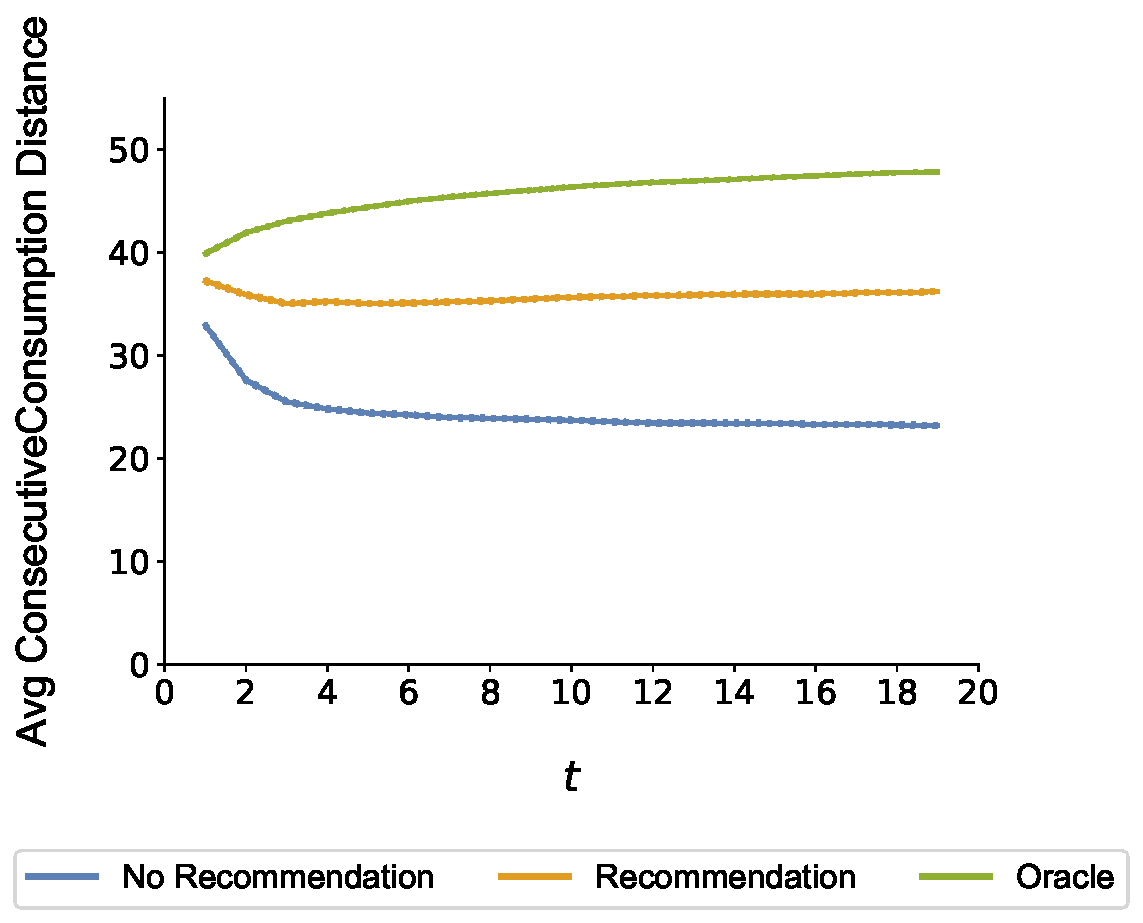
\includegraphics[width=.9\linewidth]{figures/rho_pos_consumption_dist_N_200T_20_overall.pdf}
  \label{fig:sfig1}
\end{subfigure}%
\begin{subfigure}{.5\linewidth}
  \centering
  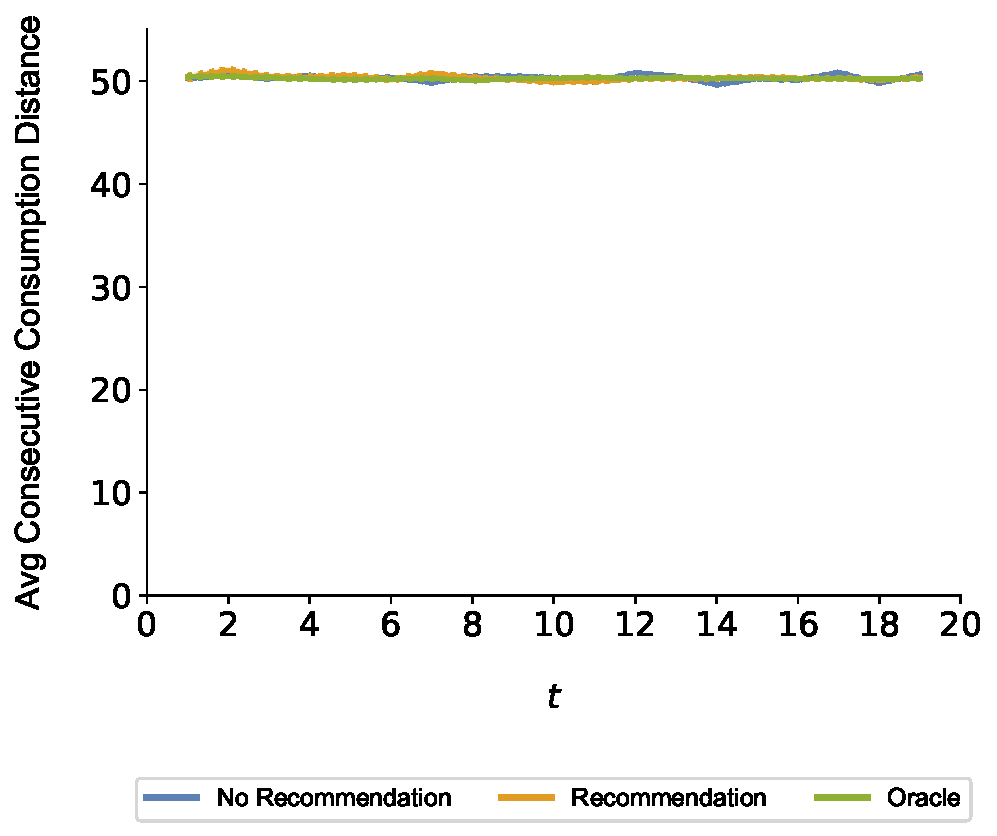
\includegraphics[width=.9\linewidth]{figures/rho_zero_consumption_dist_N_200T_20_overall.pdf}
  \label{fig:sfig2}
\end{subfigure}
\caption{Consumption path with (Left) and without (Right) correlation between values}
\label{fig:correlation_consumption_path}
\end{figure}

\section{Results}
\subsection{Local Consumption and Filter Bubbles}
We characterize ``filter bubble'' effects in our model as the degree to which users engage in \textit{local consumption}. We define local consumption in terms of the average consumption distance between the items consumed by the users at time $t-1$ and $t$. Thus, in the context of our model, filter bubble effects arise when the average consumption distance decreases over time and, across regimes, when the overall levels are lower for a given recommendation regime compared to another.


\begin{finding}\label{finding_local_consumption}
The impact of recommendation on local consumption:
\begin{enumerate}
\item When $\rho = 0$, there is no difference in consumption distance between the three recommendation regimes.
\item When $\rho > 0$, no recommendation induces more local consumption than both recommendation and oracle regimes. This effect is amplified as $\rho$ increases as well as when users are more risk averse ($\gamma$ increases)
\end{enumerate}
\end{finding}

First, the bottom panel of Figure \ref{fig:correlation_consumption_path} shows that, when $\rho = 0$, there is no difference in consumption distance between the three regimes. This is due to the fact that when $\rho = 0$, there is no reason that items that are close in the product space should have similar values and so the optimal consumption path does not depend on the similarity of the items. However this also means that users do not learn anything about neighboring products and so there is limited path-dependence in consumption. Not only is there no difference in the levels between the three regimes, but they all have the same, flat, average consumption distance path. This underscores the fact that such concerns about filter bubbles \textit{only} arise in a world where there is correlation between the realized utility of items. If there were no correlation between the realized utilities then there would be no reason for users to consume similar items and thus no narrowing effect, regardless of the information on the true utility of the items that users had.
\par
The top panel of Figure \ref{fig:correlation_consumption_path} shows that, when $\rho > 0$, both recommendation and no recommendation lead to increasingly local consumption compared to the oracle benchmark case. Further, the average consumption path between periods is \textit{decreasing} for the no recommendation case whereas it is \textit{increasing} for the oracle case. The recommendation regime decreases the degree of local consumption, but not as much as the oracle benchmark. Due to the correlation of values, the oracle consumption path exploits this and leads to the consumption of more similar products than in the case when $\rho = 0$. However, since these spillovers also impact user learning in the no recommendation case, users \textit{over-exploit} this and increasingly consume products similar to good products that they have consumed before. This is further illustrated by Figure \ref{fig:local_consumption_across_rho} which shows how the consumption paths in the oracle and no recommendation regimes vary as $\rho$ increases.
\par

Finally, this effect is further amplified as the level of risk aversion, $\gamma$, increases. Figure \ref{fig:no_rec_risk_aversion} shows how drastically the degree of local consumption increases as $\gamma$ increases. This is due to the fact that the spillovers not only affect the mean expected belief about quality but also the degree of uncertainty. Local consumption therefore leads to users having less uncertainty about certain areas of the product space and risk aversion may lead them to increasingly consume nearby products.

\begin{figure}[t]
\begin{subfigure}{.45\textwidth}
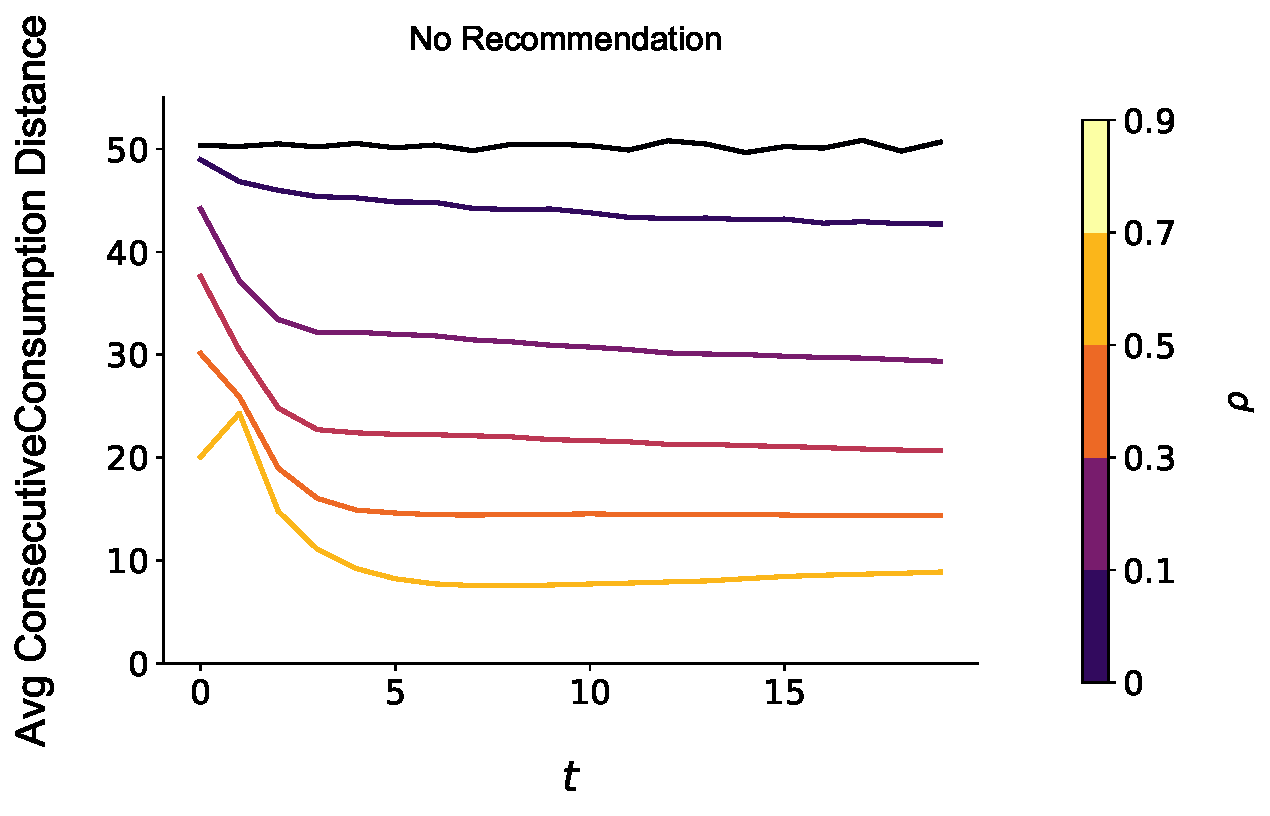
\includegraphics[width=\linewidth]{figures/rho_consumption_dist_N_200T_20.pdf}
\end{subfigure}
\begin{subfigure}{.45\textwidth}
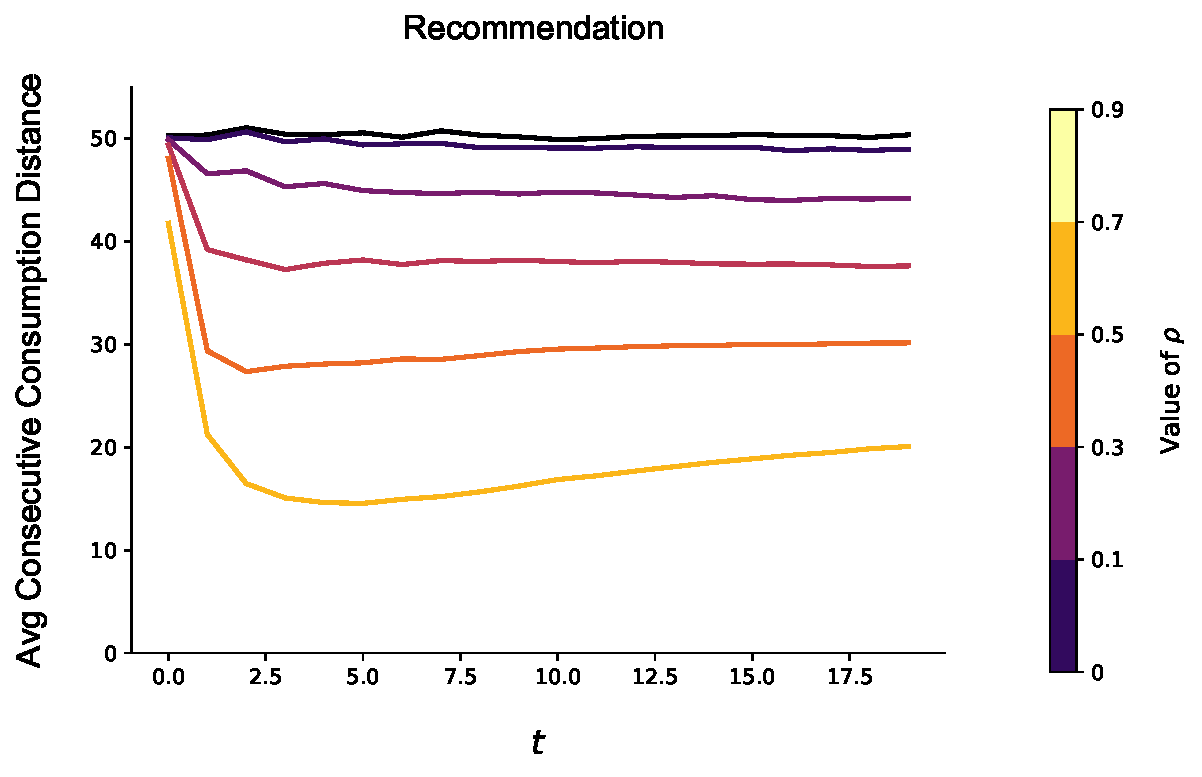
\includegraphics[width=\linewidth]{figures/rho_consumption_dist_N_200T_20_partial.pdf}
\end{subfigure}\\
\begin{subfigure}{.45\textwidth}
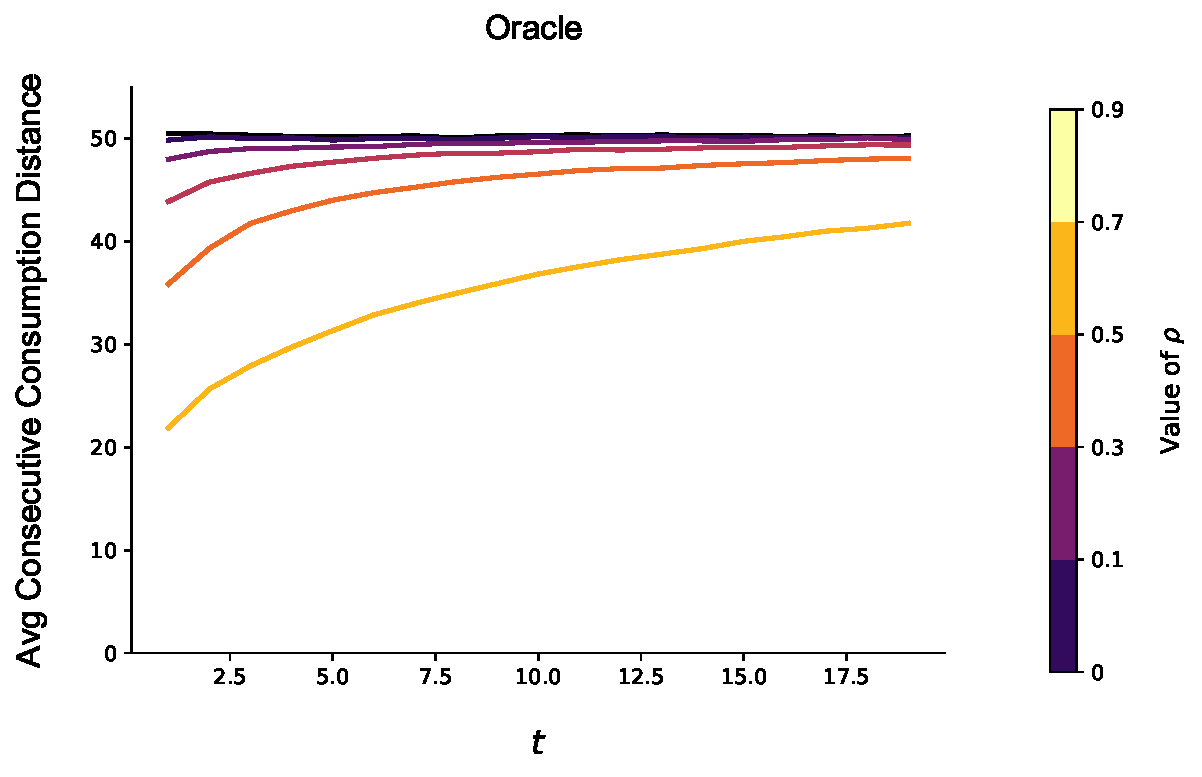
\includegraphics[width=\linewidth]{figures/rho_consumption_dist_N_200T_20_omni.pdf}\\
\end{subfigure}
\caption{Extent of Local Consumption as strength of correlation, $\rho$, varies. \\ No Recommendation (Top Left), Recommendation (Top Right) and Oracle (Bottom)}
\label{fig:local_consumption_across_rho}
\end{figure}


\begin{figure}[t]
\begin{subfigure}{.45\textwidth}
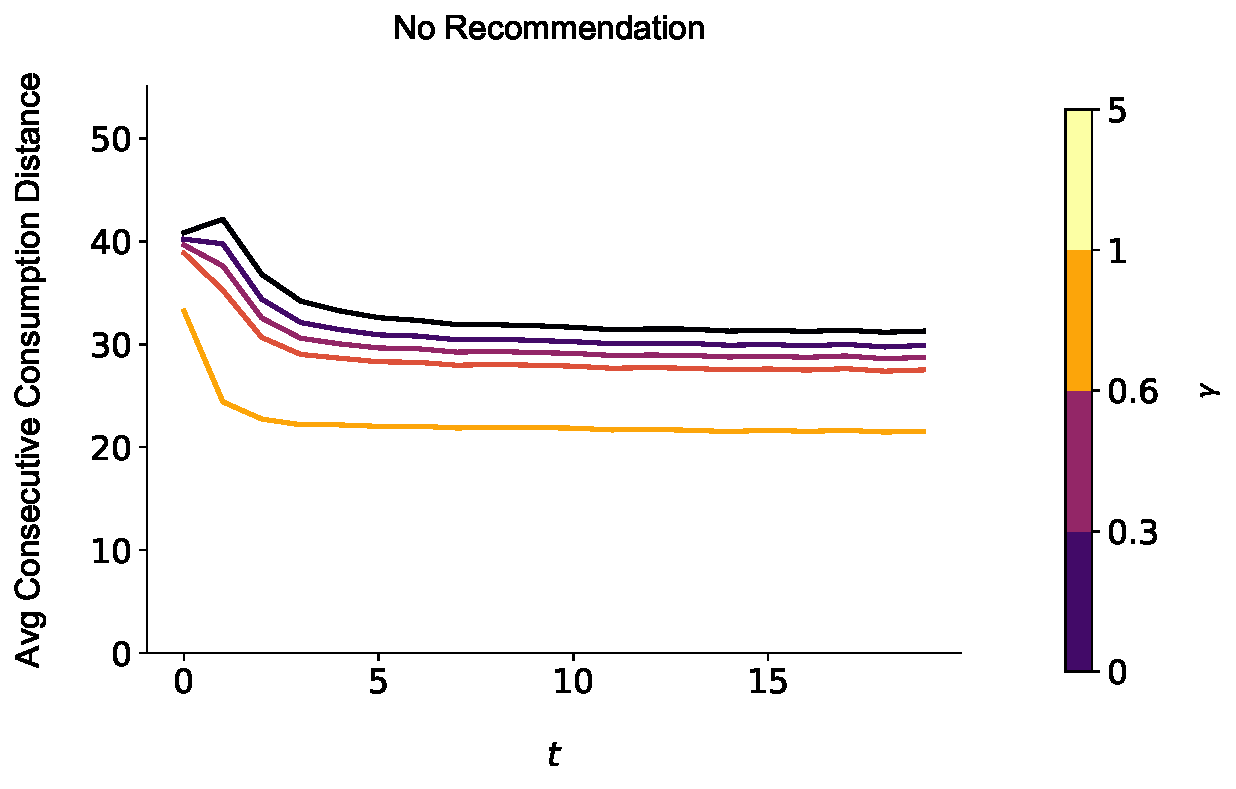
\includegraphics[width=\linewidth]{figures/gamma_consumption_dist_N_200T_20.pdf}
\end{subfigure}
\begin{subfigure}{.45\textwidth}
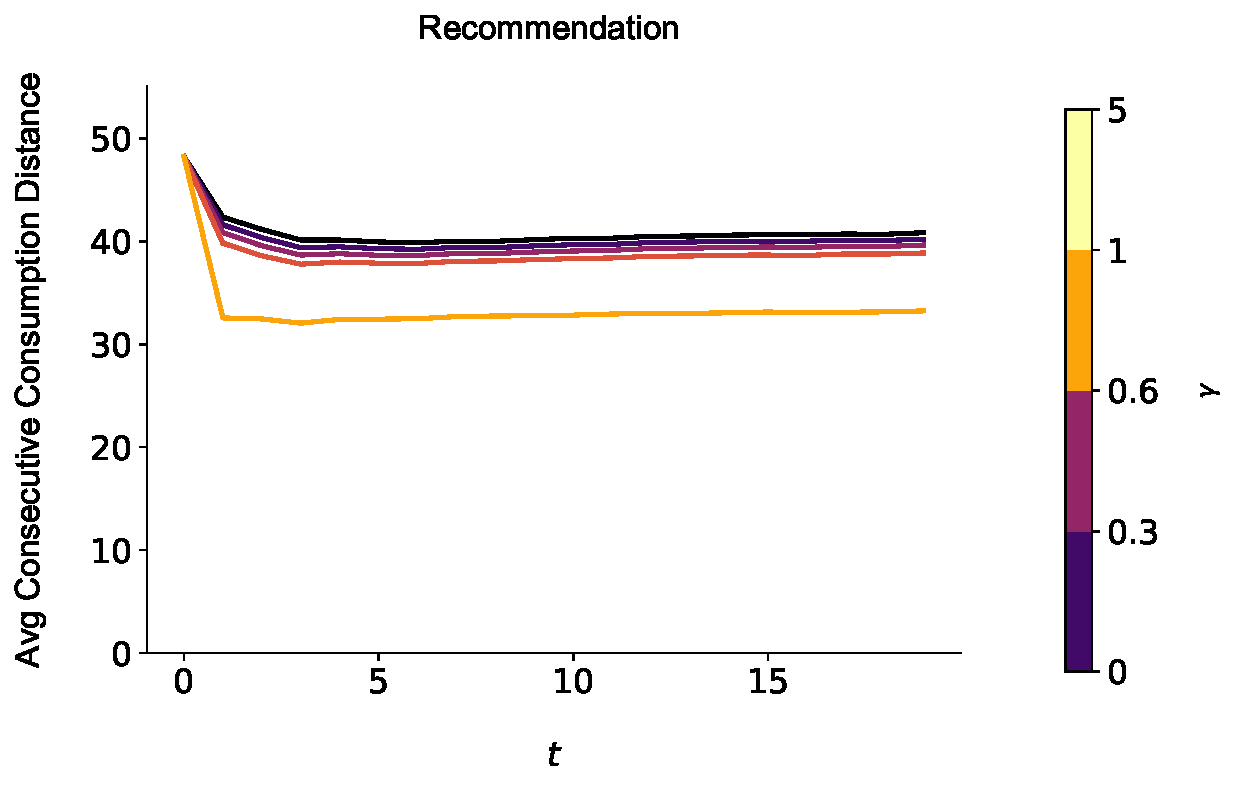
\includegraphics[width=\linewidth]{figures/gamma_consumption_dist_N_200T_20_partial.pdf}
\end{subfigure}\\
\begin{subfigure}{.45\textwidth}
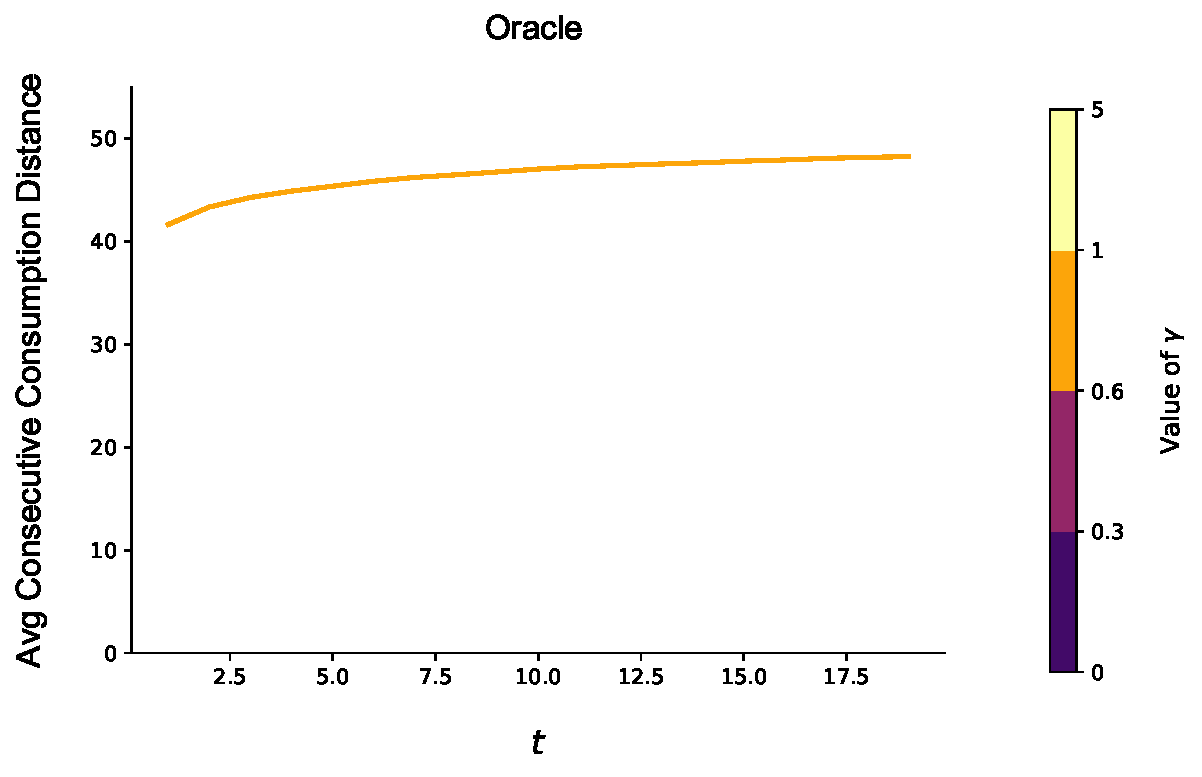
\includegraphics[width=\linewidth]{figures/gamma_consumption_dist_N_200T_20_omni.pdf}\\
\end{subfigure}%
\caption{Effect of Risk Aversion on Local Consumption \\ No Recommendation (Top Left), Recommendation (Top Right) and Oracle (Bottom)}
\label{fig:no_rec_risk_aversion}
\end{figure}

In sum, filter bubble effects can only arise when there is an inherent correlation between the realized utilities of the items in the product space. However, this is often the case in most environments where recommender systems are deployed. When there is a correlation between the realized utilities then filter bubbles can naturally arise due to the nature of how individuals acquire additional information about the remaining items. We have shown that, unless users are provided with additional information to guide their consumption choices, then these information spillovers and user risk-aversion can lead users into filter bubbles. When users consume high valued items, they exploit the underlying correlation across different products' values, stronger for similar products, which leads them to increasingly consume products in narrower and narrower portions of the product space. Risk aversion may lead users into performing local consumption even when they have a low valuation of nearby items just because they know what to expect from the item. Recommendation leads to these effects being mitigated by providing users with additional information on products outside the already explored portions of the product space. Further, if all uncertainty was resolved as in the oracle regime, then such behavior is not present.

\subsection{User Welfare and Product Diversity}
In this section we primarily focus on the impact of recommendation on user welfare and the overall diversity of the items that they consume.
\par 
While in the previous section we looked at the distance between consecutive items, in this section we focus on a diversity measure that considers the entire consumed set of items. The diversity measure we utilize is common in recommender system literature (e.g. \cite{ziegler2005improving}) which is the average normalized pairwise distance between the consumed products:
$$D_i:=\frac{1}{N}\frac{1}{T(T-1)}\sum_{n,m \in C_i^T: n \ne m} d(n,m)$$

\begin{figure}[ht]
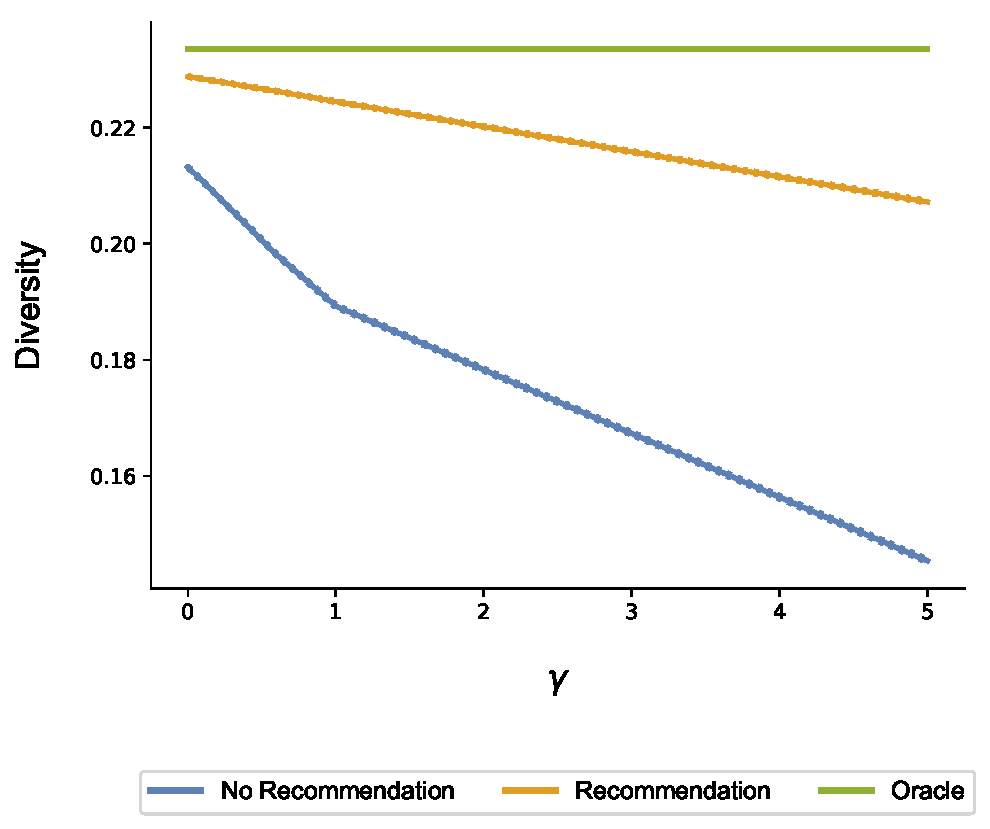
\includegraphics[width=.45\linewidth]{figures/gamma_diversity_N_200_T_20}
\captionof{figure}{Risk Aversion and Diversity}\label{fig:risk_aversion_diversity}
\end{figure}


\begin{finding}\label{finding_diversity}
The impact of recommendation on product diversity:
\begin{enumerate}
\item When $\rho = 0$, product diversity is the same across all three recommendation regimes;
\item When $\rho > 0$, product diversity decreases across all recommendation regimes but decreases the most in the no recommendation regime. This effect is amplified as $\rho$ increases as well as when users become more risk-averse.
\end{enumerate}
\end{finding}
\par 
Finding~\ref{finding_diversity} summarizes the main results on product diversity. As before, when there is no correlation between valuations, product diversity is the same across different recommendation regimes. The over-exploitation of information spillovers when $\rho > 0$ leads to product diversity being lowest in the no recommendation regime. As a result, this effect gets amplified as $\rho$ increases, which leads to the gap in diversity between the regimes to increase as $\rho$ increases. Figure \ref{fig:diversity_welfare_correlation} shows how diversity varies as $\rho$ increases across the three regimes that we consider. There is a similar increasing diversity gap as $\gamma$, or the level of risk-aversion, increases as can be seen in Figure \ref{fig:risk_aversion_diversity}. The mechanisms behind these effects have direct parallels to those discussed in the previous section since low average sequential consumption distance directly leads to low diversity.
\par 
We now study how recommendation impacts user welfare in our model. In our model users make consumption decisions that maximize their current period ex-ante utility that depends on their beliefs in that period. Thus, from an ex-ante perspective, they make optimal decisions, but our primary interest is in understanding how the ex-post, or realized, utility varies across regimes and parameter values. We define user's \textit{ex-post} welfare as the average of the realized values, controlling for the effect of $T$:
$$W_i:= \frac{1}{T}\sum_{n \in C_i^T} x_{i,n}$$

\begin{finding}\label{finding_welfare_gap}
The impact of recommendation on consumer welfare is as follows:
\begin{enumerate}
\item Under oracle recommendation, welfare is constant as $\rho$ increases.
\item Under no recommendation, welfare is increasing as $\rho$ increases.
\item Recommendation introduces welfare gains relative to no recommendation, but these gains are decreasing as $\rho$ increases. 
\end{enumerate}
\end{finding}
\par 
Finding~\ref{finding_welfare_gap} states our main findings of the impact of recommendation on ex-post welfare, which are drawn from Figure~\ref{fig:diversity_welfare_correlation}. The most interesting observation is that the value of recommendation decreases as $\rho$ decreases. The intuition for this is clear as recommendation provides users with information that allows them to better guide their decisions and increase welfare. However, as $\rho$ increases users get increasingly more information simply from consuming items since the realized utility is now more informative about the utility of nearby items. Thus, since consumption decisions themselves reveal information, the information that recommendation reveals provides less value.
\par 
Figure~\ref{fig:diversity_welfare_common_value} shows how diversity and welfare vary across recommendation regimes as the the strength of the common-value component, $\beta$, varies. As expected, when $\beta = 0$, these values are the same. However, as $\beta$ grows the idiosyncratic component of user valuations becomes increasingly less important and the recommendation regime begins to converge to the oracle regime. Indeed, we see that both product diversity and welfare increase under recommendation, whereas under no recommendation we see that there is a decrease in diversity with little changes to consumer welfare. This is intuitive as $\beta$ controls the informativeness of recommendation about user preferences.
\par 
One striking observation is that the decrease in diversity does not appear to be associated with a decline in welfare. Indeed, it appears that the opposite is the case - that low diversity is associated with higher welfare and vice versa. Thus, we next explore the relationship between welfare and diversity.
\begin{figure}
\begin{subfigure}{.45\linewidth}
  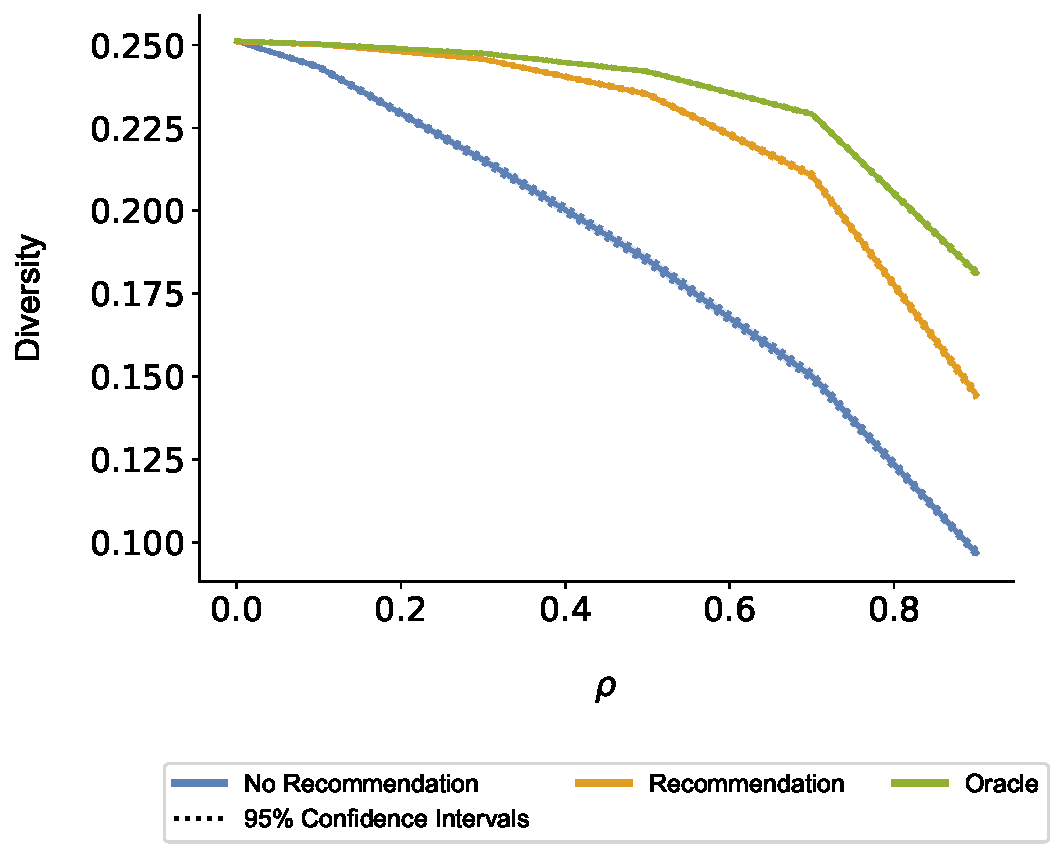
\includegraphics[width=.8\linewidth]{figures/rho_diversity_N_200_T_20.pdf}
\end{subfigure}
\begin{subfigure}{.45\linewidth}
  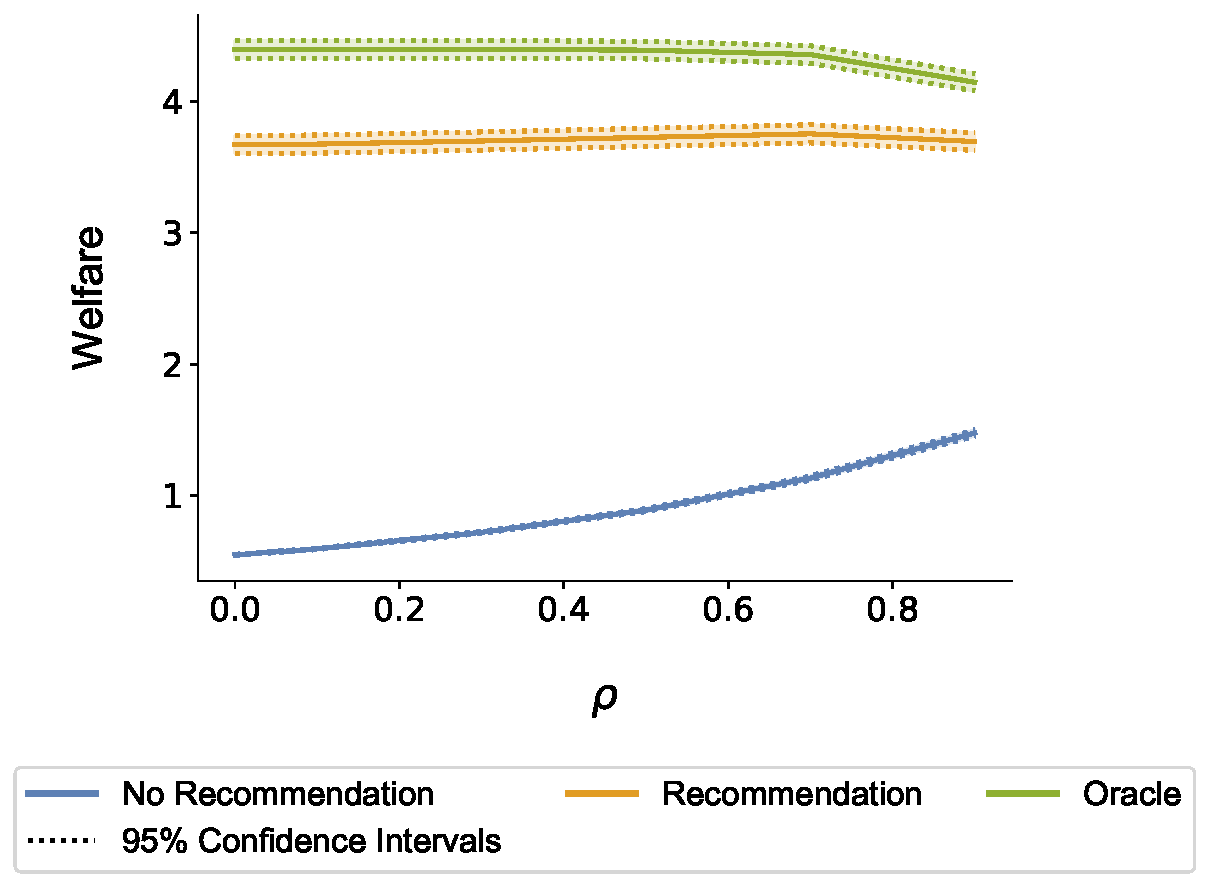
\includegraphics[width=.8\linewidth]{figures/rho_welfare_N_200_T_20.pdf}
\end{subfigure}
\caption{User Welfare and Diversity as the strength of correlation, $\rho$, varies}\label{fig:diversity_welfare_correlation}
\end{figure}

\begin{figure}
\begin{subfigure}{.45\linewidth}
  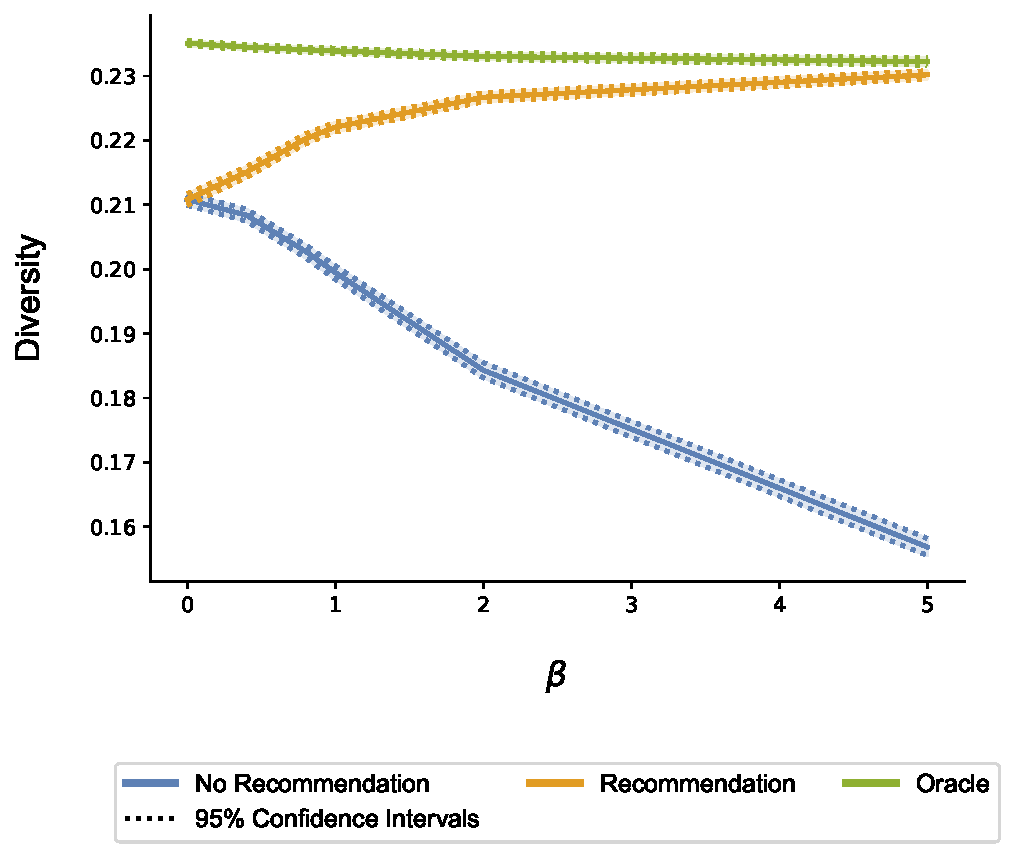
\includegraphics[width=.8\linewidth]{figures/beta_diversity_N_200_T_20.pdf}
\end{subfigure}
\begin{subfigure}{.45\linewidth}
  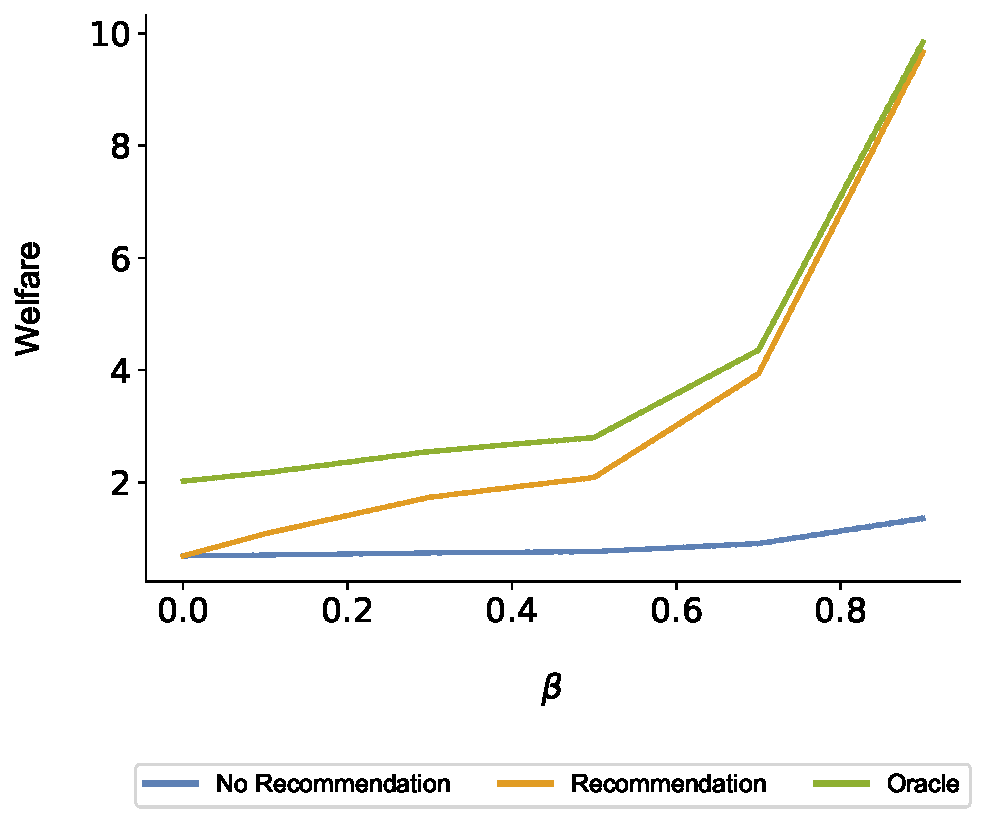
\includegraphics[width=.8\linewidth]{figures/beta_welfare_N_200_T_20.pdf}
\end{subfigure}
\caption{User Welfare and Diversity as the strength of the common value component, $\beta$, varies}\label{fig:diversity_welfare_common_value}
\end{figure}


\begin{finding}\label{finding_diversity_welfare_corr}
In the no recommendation regime, diversity and welfare are:
\begin{enumerate}
\item Negatively correlated when users have no risk-aversion;
\item Uncorrelated when users have high levels of risk-aversion.
\end{enumerate}
In the recommendation regime, diversity and welfare are:
\begin{enumerate}
\item Uncorrelated when users have no risk-aversion;
\item Positively correlated when users have high levels of risk-aversion.
\end{enumerate}
In the oracle regime, diversity and welfare are always uncorrelated.
\end{finding}

Finding~\ref{finding_diversity_welfare_corr} summarizes our findings on the relationship between diversity and welfare. Figure \ref{fig:diversity_welfare_ra} shows how diversity and welfare correlate for the no recommendation case as we vary the degree of risk aversion. When there is no risk-aversion then there is a negative correlation between welfare and diversity. This is since, with no risk-aversion, in a given period a user will select the good that she currently believes has the highest expected value. High product diversity in this case can arise from a user who consumes an item she disliked and updates her beliefs about nearby items negatively. As a result, in the following period she will pick an item far away in the product space from the item that was previously consumed. If instead the user valued highly the item that she had consumed, then she is more likely to pick a nearby item. The information spillovers therefore lead to high product diversity being negatively correlated with welfare.
\par
This only happens since $\gamma = 0$ leads to users only caring about the expected value of the product. However, as we saw in Findings \ref{finding_local_consumption} and \ref{finding_diversity}, increasing $\gamma$ can lead to lower diversity and increasingly local consumption due to the fact that the degree of uncertainty now impacts users' choices. This weakens the negative relationship between diversity and welfare since both negative and positive experiences with a good reduce uncertainty about surrounding items. This leads to the inverted-U shape found in Figure \ref{fig:diversity_welfare_ra} when $\gamma$ is relatively large (e.g $\gamma = 5$) though diversity and welfare are virtually uncorrelated in the data. In the recommendation and oracle regimes, under risk neutrality ($\gamma=0$), welfare and diversity and uncorrelated, while under risk aversion ($\gamma=5$), it is possible to observe in Figure \ref{fig:diversity_welfare_ra_partial} an actual positive relation between diversity and welfare as recommendations are able to reduce uncertainty and facilitate exploration of the product space.
\begin{figure}[t]
\begin{subfigure}{.45\textwidth}
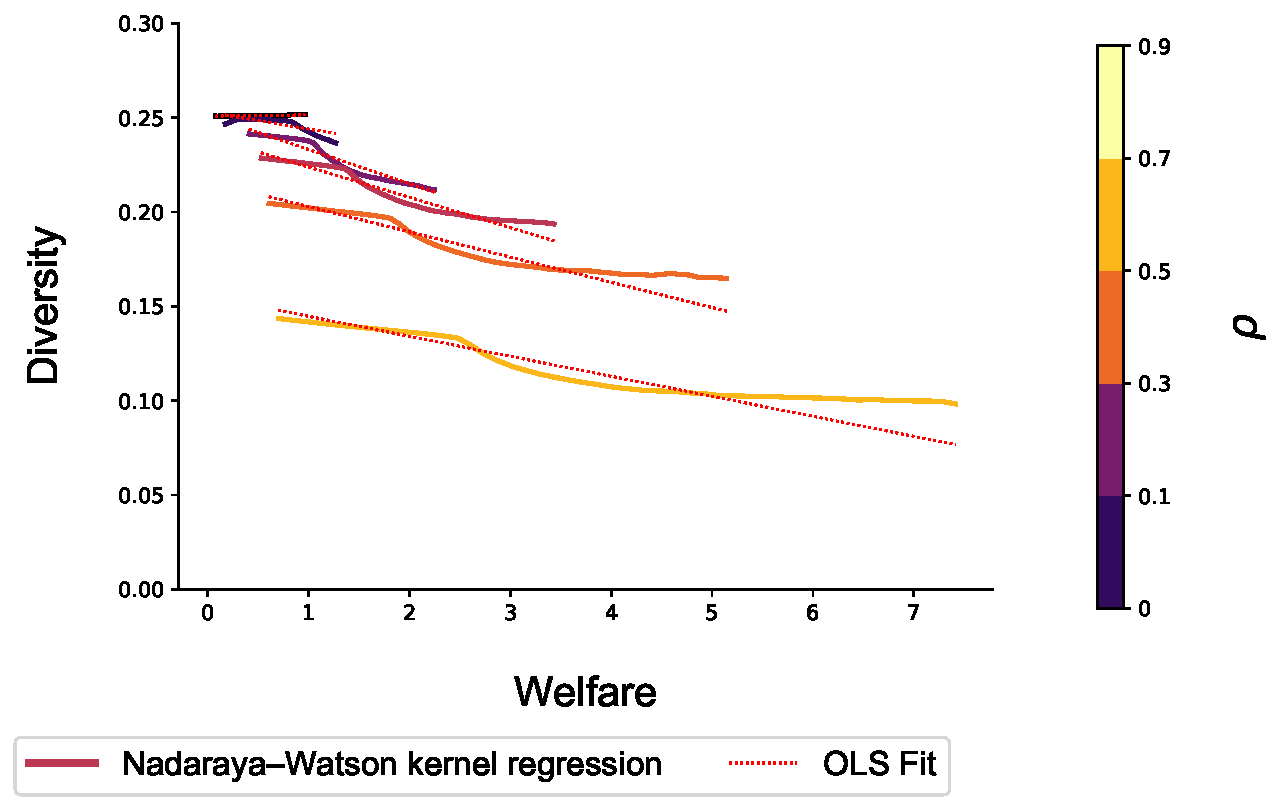
\includegraphics[width=1.05\linewidth]{figures/diversity_welfare_rn.pdf}
\end{subfigure}
\begin{subfigure}{.45\textwidth}
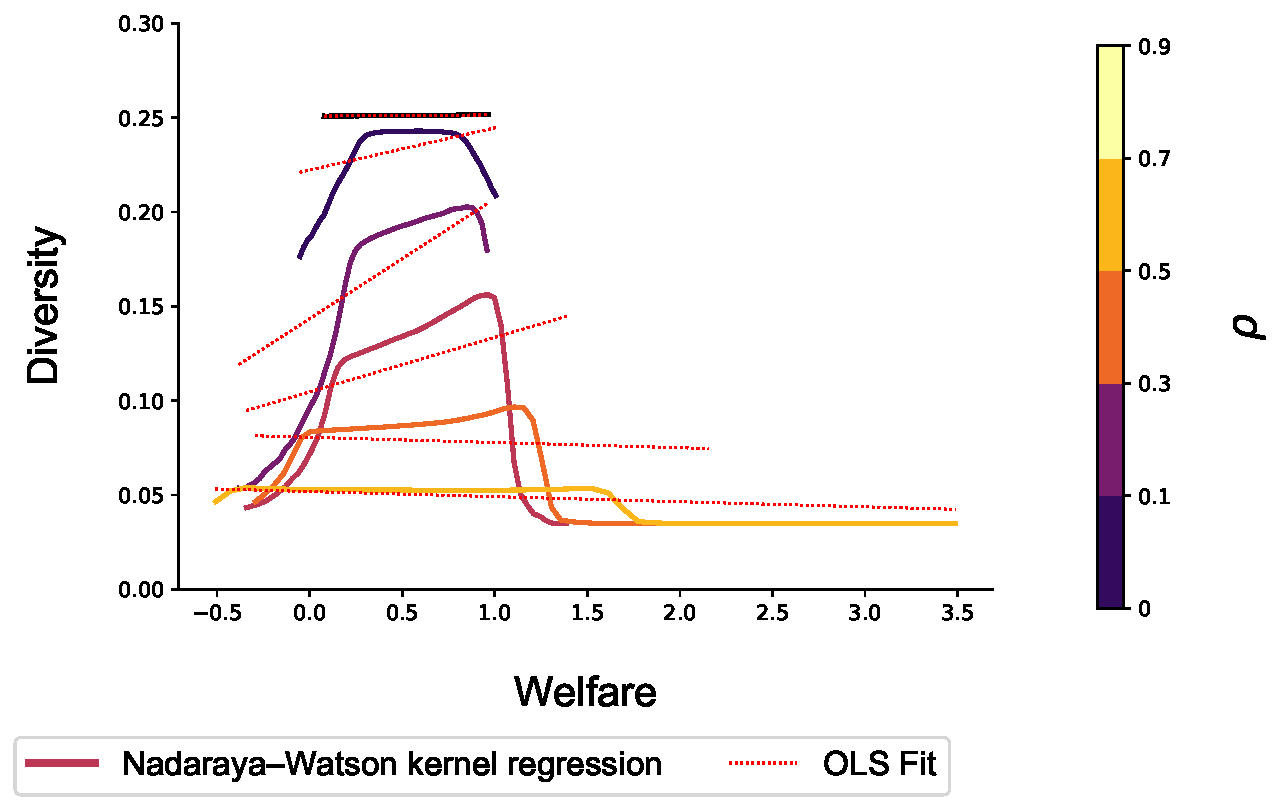
\includegraphics[width=1.05\linewidth]{figures/diversity_welfare_ra.pdf}
\end{subfigure}\\
\caption{Diversity vs. Welfare, \textbf{No-Recommendation}, $\gamma = 0$ (Left), Diversity vs. Welfare, $\gamma = 5$ (Right)}\label{fig:diversity_welfare_ra}
\end{figure}

\begin{figure}[t]
\begin{subfigure}{.45\textwidth}
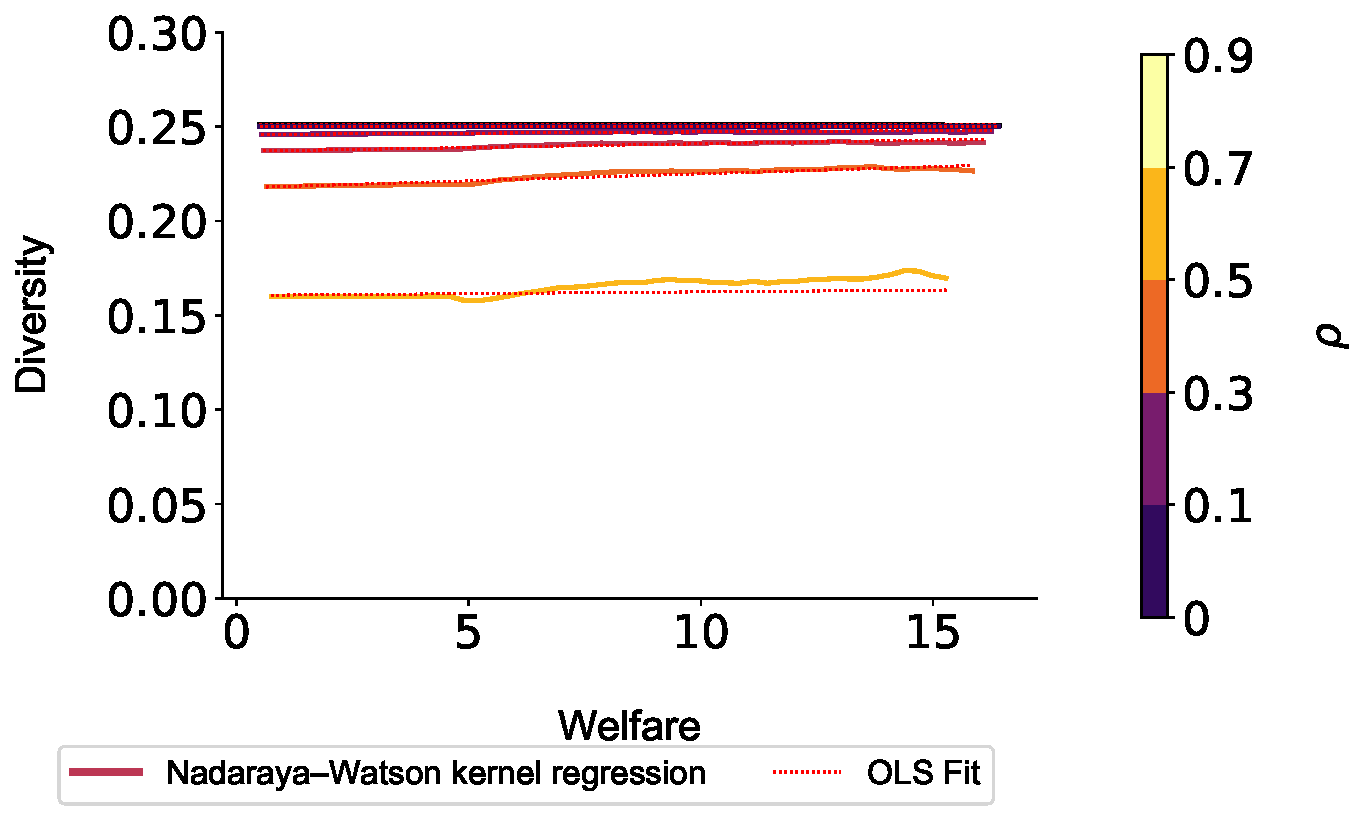
\includegraphics[width=1.05\linewidth]{figures/diversity_welfare_rn_partial.pdf}
\end{subfigure}
\begin{subfigure}{.45\textwidth}
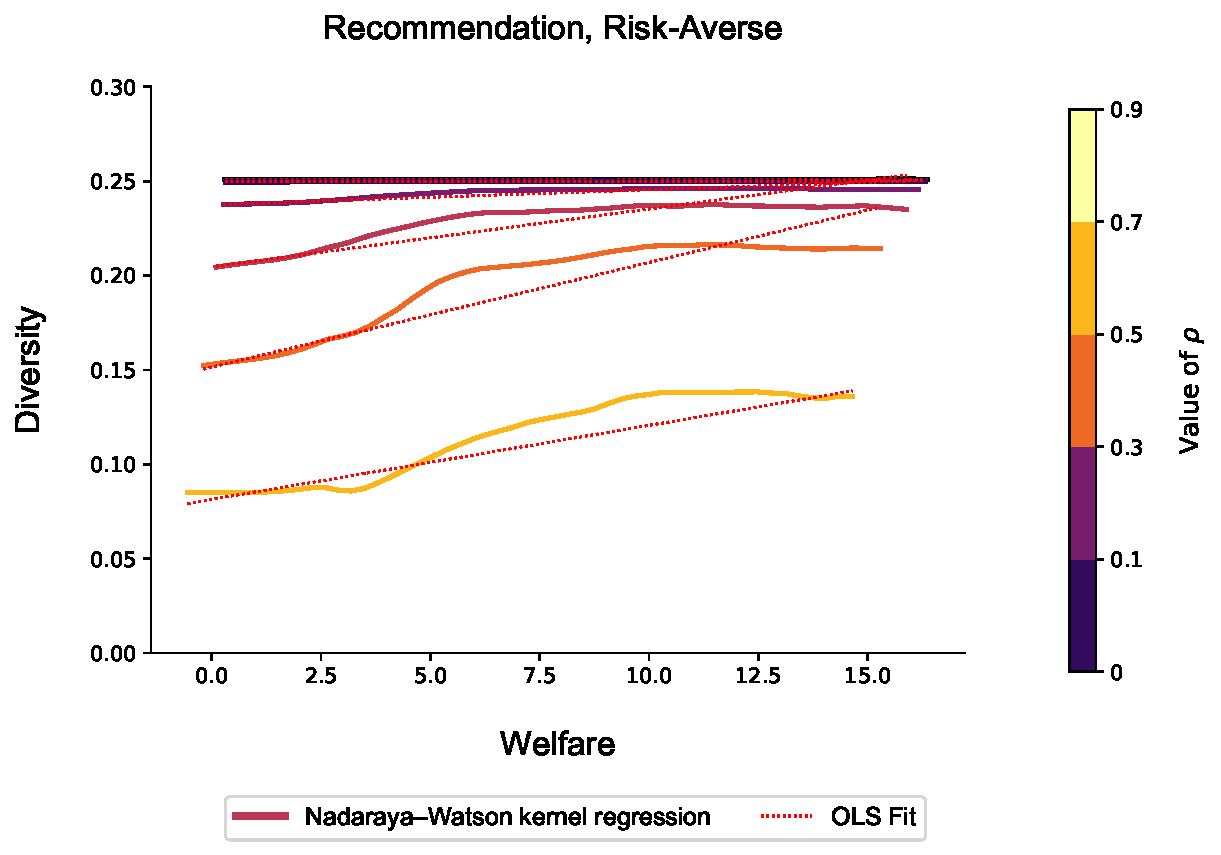
\includegraphics[width=1.05\linewidth]{figures/diversity_welfare_ra_partial.pdf}
\end{subfigure}\\
\caption{Diversity vs. Welfare, Recommendation, $\gamma = 0$ (Left), Diversity vs. Welfare, $\gamma = 5$ (Right)}\label{fig:diversity_welfare_ra_partial}
\end{figure}

\subsection{User Homogenization}
In this section, we focus on comparisons across users and investigate how the consumed set of items across users varies across different recommendation regimes and parameter values. In particular we look at the degree of \textit{homogenization} between users. Similar to other papers that study the degree of homogenization in recommender systems (e.g. \cite{chaney2018algorithmic}) we measure homogeneity via the Jaccard index between the consumption sets of users:
\begin{align*}
H:=\frac{1}{|I|(|I|-1)}\sum_{i,j \in I: i \ne j}d_J(C_i^T,C_j^T)
\end{align*}
where $d_J$ denotes the Jaccard index and $H \in [0,1]$.
\begin{finding}\label{finding_homogeneity}
The impact of recommendation on homogeneity is as follows:
\begin{enumerate}
\item Highest under recommendation and lowest under no recommendation;
\item Increasing in $\beta$, or the weight of the common-value component;
\item Decreasing in $\rho$ for partial recommendation, but weakly increasing in $\rho$ for no recommendation.
\end{enumerate}
\end{finding}
Finding~\ref{finding_homogeneity} summarizes our findings on the impact of recommendation on user homogeneity. First, we study how the degree of homogenization varies as we increase $\beta$, the weight of the common value component. As $\beta$ increases we expect that users should become increasingly homogeneous as the realized utilities of the items are now increasingly similar. Figure \ref{fig:beta_homo} confirms that as the weight of the common-value component, $\beta$, increases users consume increasingly similar sets of items. The homogenization effect is strongest under the recommendation regime since the revelation of the common-value component induces users to consume products in similar areas of the product space. As $\beta$ increases, some amount of homogenization is optimal as can be seen from the oracle case. However, since users in the no recommendation regime do not know the common-value component they engage in local consumption in different areas of the product space which leads to less than optimal homogeneity.
\par
We next study how the degree of homogeneity varies as $\rho$ increases. Figure \ref{fig:cor_homo} shows how homogeneity varies as $\rho$ increases across the different recommendation regimes. The most striking finding is that homogeneity decreases as $\rho$ increases in the recommendation regime. As was highlighted in Findings \ref{finding_local_consumption} and \ref{finding_diversity}, the degree of local consumption increases with $\rho$. Even though the revelation of the common-value component induces them to search in similar parts of the product space, their idiosyncratic components induce them to consume products in a more localized area of the product space as $\rho$ increases which leads to a decline in homogeneity.

\begin{figure}[t]
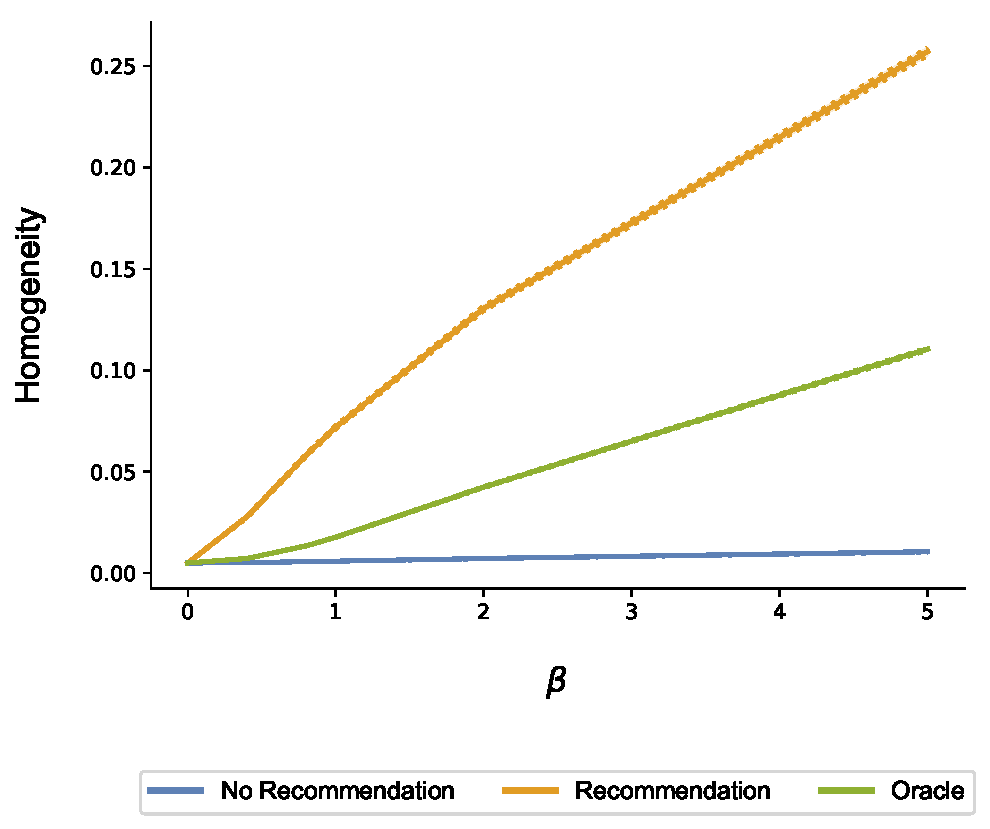
\includegraphics[width=.45\linewidth]{figures/beta_homogeneity_N_200_T_20}
\captionof{figure}{Strength of Recommendation and Homogeneity}\label{fig:beta_homo}
\end{figure}
~

\begin{figure}[t]
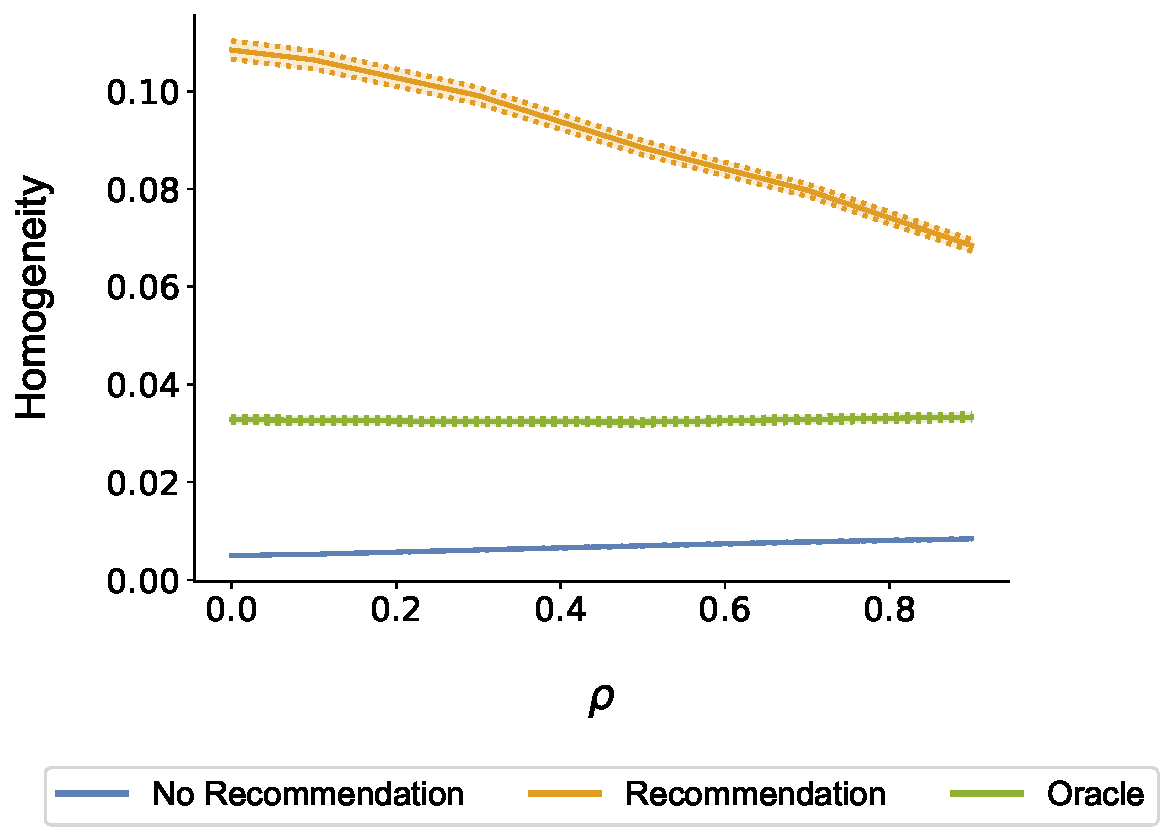
\includegraphics[width=.45\linewidth]{figures/rho_homogeneity_N_200_T_20}
\captionof{figure}{Correlation and Homogeneity}\label{fig:cor_homo}
\end{figure}

\section{Conclusion}
We have studied a model of user decision-making in the context of markets where recommender systems are traditionally deployed in order to understand the consequences of recommender systems on consumption patterns of users. The key components of the model are that users make decisions under uncertainty and that consuming a good leads to informational spillovers about similar items. We have shown that this alone can generate consumption behavior that is consistent with filter bubble effects that have traditionally been associated with personalized recommender systems. This effect is weakened once we allow for recommendation, but not as much as if users have full information. We have further explored the relationship between consumption diversity and user welfare and found that they are negatively correlated, implying that striving for consumption diversity is not necessarily welfare-improving for users. Finally, we have shown that recommendation can lead to increases in user homogenization both relative to no recommendation and full information since it concentrates users' consumption in portions of the product space with the highest utility according to the limits of what the recommender can predict about the utility of the good.
\par 
Our results highlight that user choice in these markets is path dependent as a result of the nature of user preferences and how these preferences evolve over time. This has important ramifications for understanding the extent to which recommender systems can steer user behavior, potentially in anti-competitive ways. Steering users towards certain items today provides them with information that they utilize to make decisions tomorrow, which leads them to consume similar items to those they were originally steered towards. Thus, online platforms can potentially shape the long-term preferences of users and not only impact their current period choices. This has broader ramifications about the equilibrium effects of such behavior on competition and consumer welfare in online platforms which we leave to future work.
\par
We leave for future work exploring to what extent user behavior changes if we drop the myopia assumption, so that users themselves are engaging in explicit exploration. This likely interacts with recommendation in interesting ways as the recommendations may provide information that can complement or crowd-out user-led exploration. Even under the myopia assumption, understanding which recommendation system is optimal is an interesting and challenging problem. Further, our results point to an important consideration in the literature on incentivizing exploration which is that the exploration faced by the recommender itself likely interacts in interesting and important ways with the choice problem faced by the users.
\par 
Overall, understanding how users make choices in online platforms and how recommender systems impact these choices is important to understand. Understanding these issues allows us to better understand the broader social and economic impact of such systems as well as can provide a guide to the improved design of such systems.
% Bibliography
\bibliographystyle{ACM-Reference-Format}
\bibliography{refs}

\end{document}
